% Définition du nom du chapitre
\chapter[Monitoring marine habitats with underwater photogrammetry: a cost-effective, accurate, precise and high-resolution reconstruction method]{Chapitre 2: Monitoring marine habitats with underwater photogrammetry: a cost-effective, accurate, precise and high-resolution reconstruction method} \label{chapitre2-methode}

\pagestyle{main}

%%%%%%%%%%%%%%%%%%%%%%%%%%%%%
%%% Figure cover chapitre %%%
%%%%%%%%%%%%%%%%%%%%%%%%%%%%%
\begin{center}
\begin{tikzpicture}
  \def\ig{%
   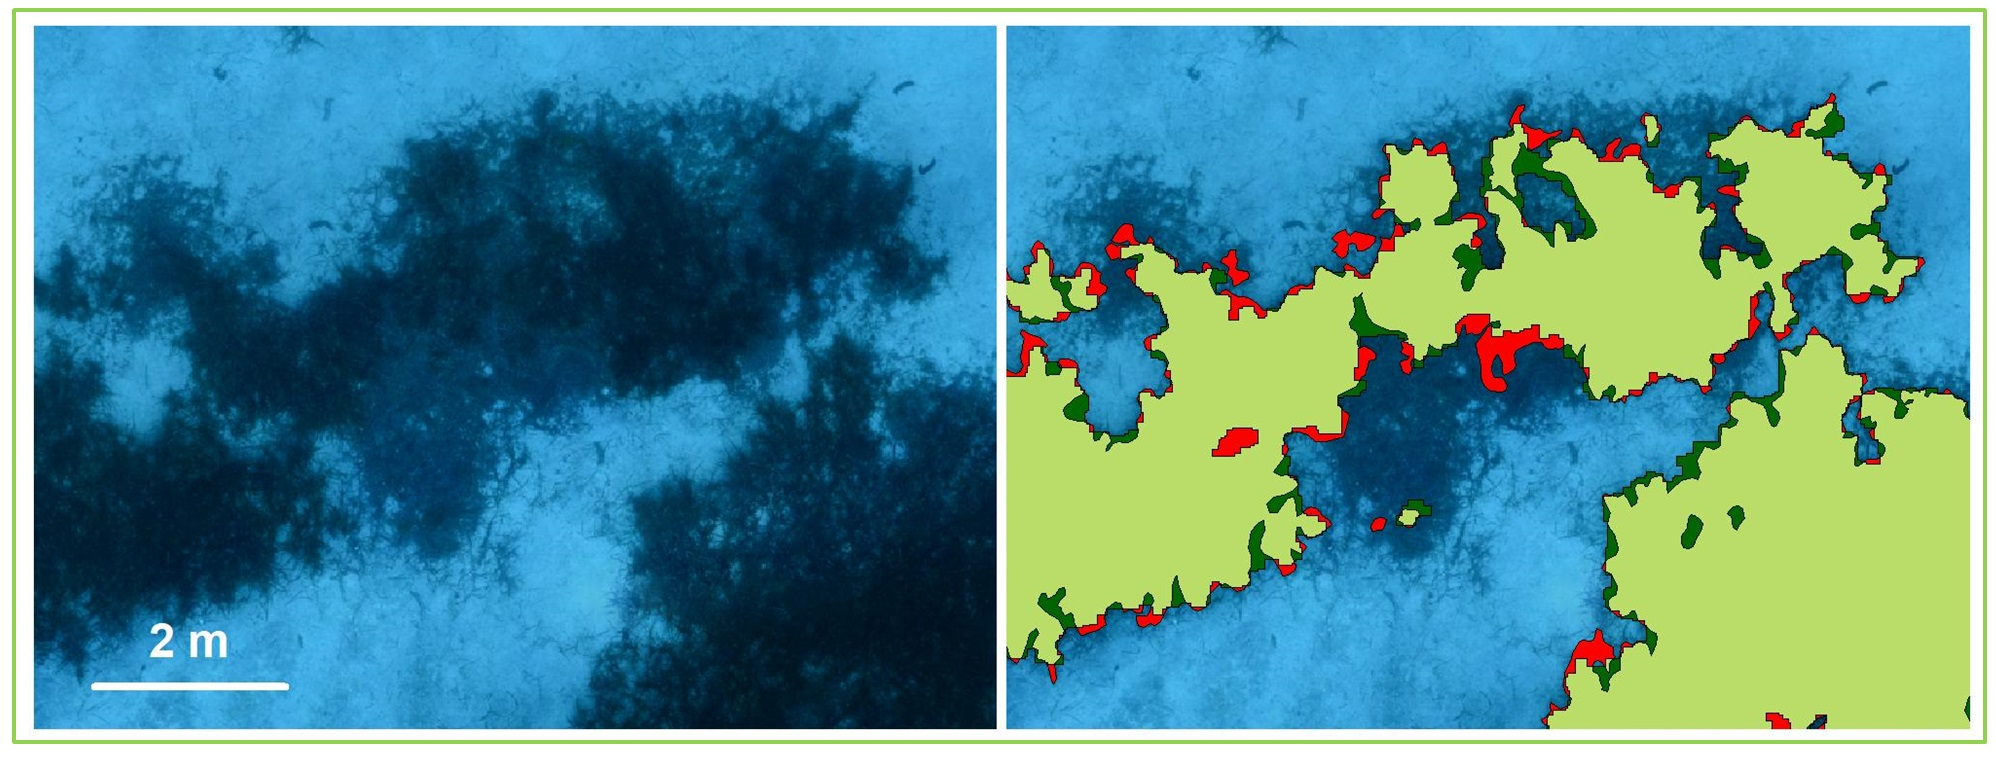
\includegraphics[width=\linewidth,keepaspectratio]{./4_chapitre2/cover.jpg}}
 \node [inner sep=0pt](mypicture) at (0,0) {\phantom{\ig}};
 \clip[rounded corners=5mm] ($(mypicture.south west)+(\bord,\bord)$) rectangle ($(mypicture.north east)-(\bord,\bord)$);
 \node[inner sep=0pt](mypicture) at (0,0) {\ig};
\end{tikzpicture}
\end{center}


% Bullet points du début de chapitre
\begin{center}
\begin{colbox}{resume}
  \vspace{-2pt}
{\color{textresume}\small
\begin{itemize}[leftmargin=0in]\itemsep3pt
\item \textbf{OBJECTIFS}~:
    \begin{itemize}
      \item Définir une méthode \textbf{standardisée} et \textbf{optimale} d'acquisition des modèles 3D~;
      \item Quantifier la \textbf{précision} des reconstructions produites avec cette méthode~;
    \end{itemize}
\item \textbf{RESULTATS}~:
    \begin{itemize}
      \item La \textbf{distance à l'objet} et la \textbf{résolution} de l'appareil photo influencent fortement la \textbf{résolution} des modèles~;
      \item La \textbf{densité} de photos influence la \textbf{qualité de l'alignement} et la \textbf{durée totale} des calculs~;
      \item Avec le meilleur protocole, la résolution moyenne des modèles est de \textbf{3.4 mm}, la propagation d'erreur de l'ordre du \textbf{mm / m} en XYZ, et les erreurs de mesures \textbf{< 1 \%}.
    \end{itemize}
\end{itemize}
}
\vspace{-2pt}
\end{colbox}
\end{center}

\clearpage

\fontsize{14}{14}{\noindent\textbf{Monitoring marine habitats with underwater photogrammetry: a cost-effective, accurate, precise and high-resolution reconstruction method}}
\normalsize
\medskip

% Auteurs
%\noindent Guilhem Marre, Florian Holon, Sandra Luque, Pierre Boissery et Julie Deter
%\medskip

% NB sans indentation
\noindent\href{https://doi.org/10.3389/fmars.2019.00276}{\textit{Marre G, Holon F, Luque S, Boissery P and Deter J (2019) Monitoring Marine Habitats With Photogrammetry: A Cost-Effective, Accurate, Precise and High-Resolution Reconstruction Method. Front. Mar. Sci. 6:276. doi: 10.3389/fmars.2019.00276}}

\medskip

\noindent\textbf{Abstract}
Underwater photogrammetry has been increasingly used to study and monitor the three-dimensional characteristics of marine habitats, despite a lack of knowledge on the quality and reliability of the reconstructions. More particularly, little attention has been paid to exploring and estimating the relative contribution of multiple acquisition parameters on the model resolution (distance between neighbour vertices), accuracy (closeness to true positions / measures) and precision (variability of positions / measures). On the other hand, some studies used expensive or cumbersome camera systems that can restrict the number of users of this technology for the monitoring of marine habitats. This study aimed at developing a simple and cost-effective protocol able to produce accurate and reproducible high-resolution models. Precisely, the effects of the camera system, flying elevation, camera orientation and number of images on the resolution and accuracy of marine habitat reconstructions was tested through two experiments. A first experiment allowed for testing all combinations of acquisition parameters through the building of 192 models of the same 36 m\textsuperscript{2} study site. The flying elevation and camera system strongly affected the model resolution, while the photo density mostly affected bundle adjustment accuracy and total processing time. The camera orientation, in turn, mostly affected the reprojection error. The best combination of parameters was used in a second experiment to assess the accuracy and precision of the resulting reconstructions. The average model resolution was 3.4 mm, and despite a decreasing precision in the positioning of markers with distance to the model centre (0.33, 0.27 and 1.2 mm / m Standard Deviation (SD) in X, Y, Z, respectively), the measures were very accurate and precise: 0.08 \% error $\pm$ 0.06 SD for bar lengths, 0.36 \% $\pm$ 0.51 SD for a rock model area and 0.92 \% $\pm$ 0.54 SD for its volume. The 3D geometry of the rock only differed by 1.2 mm $\pm$ 0.8 SD from the ultra-high resolution in-air reference. These results suggest that this simple and cost-effective protocol produces accurate and reproducible models that are suitable for the study and monitoring of marine habitats at a small reef scale.

\medskip
\noindent\textbf{Keywords}
underwater photogrammetry, resolution, accuracy, precision, 3D habitat mapping, marine ecology

\section[Introduction]{Introduction}\label{chapitre2_1}
Mapping marine habitats on a large scale has been of primary interest for years as it is essential to estimate, to understand, and to predict biotic assemblages and the distribution of marine biodiversity \citep{tittensor_mid-term_2014}. To date, knowledge on the patterns and changes of marine biodiversity in Europe and its role in ecosystem functioning has been scattered and imprecise. In the past few years however, the study of marine biodiversity has risen from relative obscurity to becoming an important issue in European policy and science. The reason is obvious: the seas are not exempt from the impacts of the Anthropocene and the diversity of life in marine ecosystems is rapidly changing \citep{mcgill_fifteen_2015}. Nevertheless, most indicators of biodiversity loss relate to the global scale \citep{pimm_biodiversity_2014}, whereas it is locally that biodiversity needs to be monitored in order to capture a potential consistent loss, which is still not properly detected at the global scale \citep{dornelas_assemblage_2014}. Key data for studying the effects of anthropogenic pressures on the marine environment at different scales, from local to global, is in fact lacking \citep{halpern_global_2008}. Conversely, two-dimensional maps are insufficient for the understanding of fine scale ecological processes as the structural complexity of benthic habitats has been shown to play a major role in structuring their constitutive ecological assemblages \citep{agudo-adriani_colony_2016, darling_relationships_2017, friedlander_designing_2003, graham_importance_2013, kovalenko_habitat_2012}. Besides, monitoring marine habitats requires the accurate measurement of lengths, areas and volumes that are difficult or even impossible to get in situ with traditional methods. A variety of tools and techniques have been used to measure these metrics, from in situ diver measurements \citep{dustan_digital_2013} to remote sensors such as airborne Lidar (Wedding et al. 2008). These are either punctual with very low spatial resolution (distance between neighbour points / vertices), not accurate enough, or limited to very shallow waters. There is certainly a need for a cost-effective and operational, accurate (closeness of a measurement to the true value \citep{granshaw_photogrammetric_2016}), precise (low variability, highly reproducible) and high resolution three-dimensional (3D) protocol for capturing the fine-scale architecture of marine habitats.
Modern photogrammetry, also known as structure-from-motion, defines the 3D reconstruction of an object or scene from a high number of photographs taken from different points of view \citep{figueira_accuracy_2015}. Photogrammetry was first developed for terrestrial applications, and it was later introduced for underwater use by archaeologists in the 1970s \citep{drap_underwater_2012, pollio_applications_1968}. This technique has seen impressive growth during the last decade and is now extensively used in marine ecology to study interactions between habitat structure and the ecological assemblages \citep{darling_relationships_2017}. It has also been used to automatically map the seabed from metrics such as luminance \citep{mizuno_simple_2017}, and simply as a tool for monitoring growth of benthic sessile organisms \citep{abdo_efficiently_2006, bythell_three-dimensional_2001, chong_underwater_2002, gutierrez-heredia_simple_2015, holmes_estimating_2008, reichert_3d_2016}. Based on this technique, recent developments in hardware and image processing have rendered possible the reconstruction of high-resolution 3D models of relatively large areas (1 ha) \citep{friedman_multi-scale_2012, gonzalez-rivero_catlin_2014, leon_measuring_2015}. However, the underwater environment is still challenging due to many factors: no GPS information is available to help positioning the photographs, light refraction reduces the field of view and makes necessary the use of a wide angle lens that increases image distortions \citep{guo_accuracy_2016, menna_optical_2017}, and large lighting and water clarity variations affect the image quality and consequently the calculation of the position and orientation of the photographs (i.e bundle adjustment) \citep{bryson_characterization_2017}. Despite these environmental constraints, many studies showed relatively accurate 3D models reconstructed with photogrammetry, notably individual scleractinian corals (2 – 20 \% accuracy for volume and surface area measurements, depending on colony complexity) \citep{bythell_three-dimensional_2001, cocito_3-d_2003, courtney_estimating_2007, gutierrez-heredia_end_2016, lavy_quick_2015}.
Monitoring benthic biodiversity through 3D reconstruction requires a sub-centrimetric to millimetric resolution, with a corresponding accuracy (closeness to true positions / measures) and precision (variability of positions / measures). This is because some habitats are highly complex in structure and have low growth such as coral reefs \citep{pratchett_spatial_2015} or coralligenous reefs \citep{ballesteros_mediterranean_2006, garrabou_growth_2000, sartoretto_structure_1994}. In order to be able to monitor these important habitats for biodiversity, very high-resolution and accurate reconstructions to detect slow growth or small changes in structure over time are needed. Nevertheless, improve resolution and accuracy come at a cost. In this instance, the finer the resolution for a given surface area, the more time-consuming the modelling process is, and with a very high number of images the reconstruction software can even reach the machine limits \citep{agisoft_agisoft_2018-1}. Ultimately, large photogrammetric models are usually made to the detriment of the final resolution and require expensive, hard to deploy ‘Underwater Autonomous Vehicles’ (UAV) \citep{johnson-roberson_generation_2010}. There is consequently a need to strike a balance between a robust and highly accurate protocol, and a methodology that remains relatively low-cost and time-effective, in order to map numerous sites within a large-scale monitoring system. The correlation between local ecological processes, quantified on punctual 3D models, and continuous macro-ecological variables available at broader scale, could help better understand and manage marine biodiversity of entire regions \citep{gonzalez-rivero_scaling_2016}.

Over the last decade, many research teams have developed their own methodology, some using monoscopic photogrammetry \citep{figueira_accuracy_2015, gutierrez-heredia_simple_2015, burns_integrating_2015,burns_utilizing_2015, burns_assessing_2016}, and some using stereo photogrammetry \citep{abdo_efficiently_2006, bryson_characterization_2017, pizarro_simple_2017, ferrari_quantifying_2016}. Others have worked on the effect of trajectory \citep{pizarro_simple_2017}, camera orientation \citep{chiabrando_influence_2017, raczynski_accuracy_2017}, and camera system \citep{guo_accuracy_2016} on the resulting model accuracy. Others focused on the repeatability of measurements such as volume \citep{lavy_quick_2015} and surface rugosity in different environmental conditions \citep{bryson_characterization_2017}. Most of these studies had the same goal underpinning: estimating the accuracy and precision of the models and their derived metrics, and eventually assessing the effect of a given driver. If some of these effects are well documented in traditional photogrammetry, there is still a lack of knowledge on their transposition below the surface. Indeed, underwater photogrammetry remains understudied. Moreover, none of the underwater studies explicitly tested different configuration arrangements on one given study area in order to assess the relative effects of all the parameters on the model, including resolution, accuracy and precision. Knowing the best possible results in underwater conditions remains a research gap. Recently, an effort has been made to assess the influence of photo density (the number of photos per m\textsuperscript{2}) on volume-area \citep{raoult_how_2017} and rugosity measurements \citep{bryson_characterization_2017}. Although most software manuals recommend a minimum overlap between photos to ensure correct bundle adjustments and accurate models (80 \% overlap + 60 \% side-overlap (Agisoft 2018)), it proved difficult to quantify the influential factors. So far it seems that no study about underwater photogrammetry has considered either the effect of flying elevation, or the total processing time of the images as criteria for the definition of an operational and cost-effective monitoring method. These two factors are yet crucial to take into account as they are likely to affect both model resolution and the capacity to monitor numerous sites.
Based on monoscopic multi-image photogrammetry, this study aims to define an operational, cost-effective methodology of producing high-resolution models of surfaces ranging between a few square meters to 500 m\textsuperscript{2}, in order to monitor marine biodiversity of temperate and tropical habitats. This study will define a method that is easy to handle, compatible with off-the-shelf commercial softwares, with a sub-centimetric resolution and the lowest processing time possible. Through the setup of two experiments, we tested in natura the influence of the camera system, flying elevation, camera orientation and photo density on the resolution, accuracy and precision of 3D reconstructions. More particularly, this study addresses the following questions:

\newlist{inparaenum}{enumerate}{2}% allow two levels of nesting in an enumerate-like environment
% \setlist[inparaenum]{nosep}% compact spacing for all nesting levels
\setlist[inparaenum,1]{label=\bfseries\arabic*.}% labels for top level
\setlist[inparaenum,2]{label=\emph{\alph*})}% labels for second level

\begin{inparaenum}
  \item What is the relative influence of camera system, flying elevation, camera orientation and photo density on:
  \begin{inparaenum}
    \item The accuracy of bundle adjustment?
    \item The number of points in the dense cloud?
    \item The model resolution?
  \end{inparaenum}
  \item What is the best value for the photo density considering the trade-off between accurate bundle adjustment, high dense cloud size, high resolution and low processing time?
   \item Having considered the best combination of these parameters in relation to the photo density, what is the expected accuracy and precision for:
  \begin{inparaenum}
    \item The XYZ positioning of markers? 
    \item The measures of length, area and volume?
    \item The reconstruction of 3D geometries?
  \end{inparaenum}
\end{inparaenum}

\section{Materials and methods}\label{chapitre2_2}

Two experiments were carried out. The first experiment (hereafter referred to as “experiment 1”) entailed testing all combinations of the parameters and assessing their relative effects on the accuracy of the bundle adjustment and model resolution. The second experiment (hereafter “experiment 2”) entailed measuring the accuracy and precision of the models, reconstructed with the best combination of parameters found in experiment 1. The process flow diagram is illustrated in Figure \ref{figure2.1}.

%%%%%%%%%%%%%%%%%%%%%%%%%%%%%%%%%%%%%%%%%%%%%%%%%%%
%%% Figure 2.1: Flow diagram of the methodology %%%
%%%%%%%%%%%%%%%%%%%%%%%%%%%%%%%%%%%%%%%%%%%%%%%%%%%
\begin{figure}[H]
	\begin{center}
	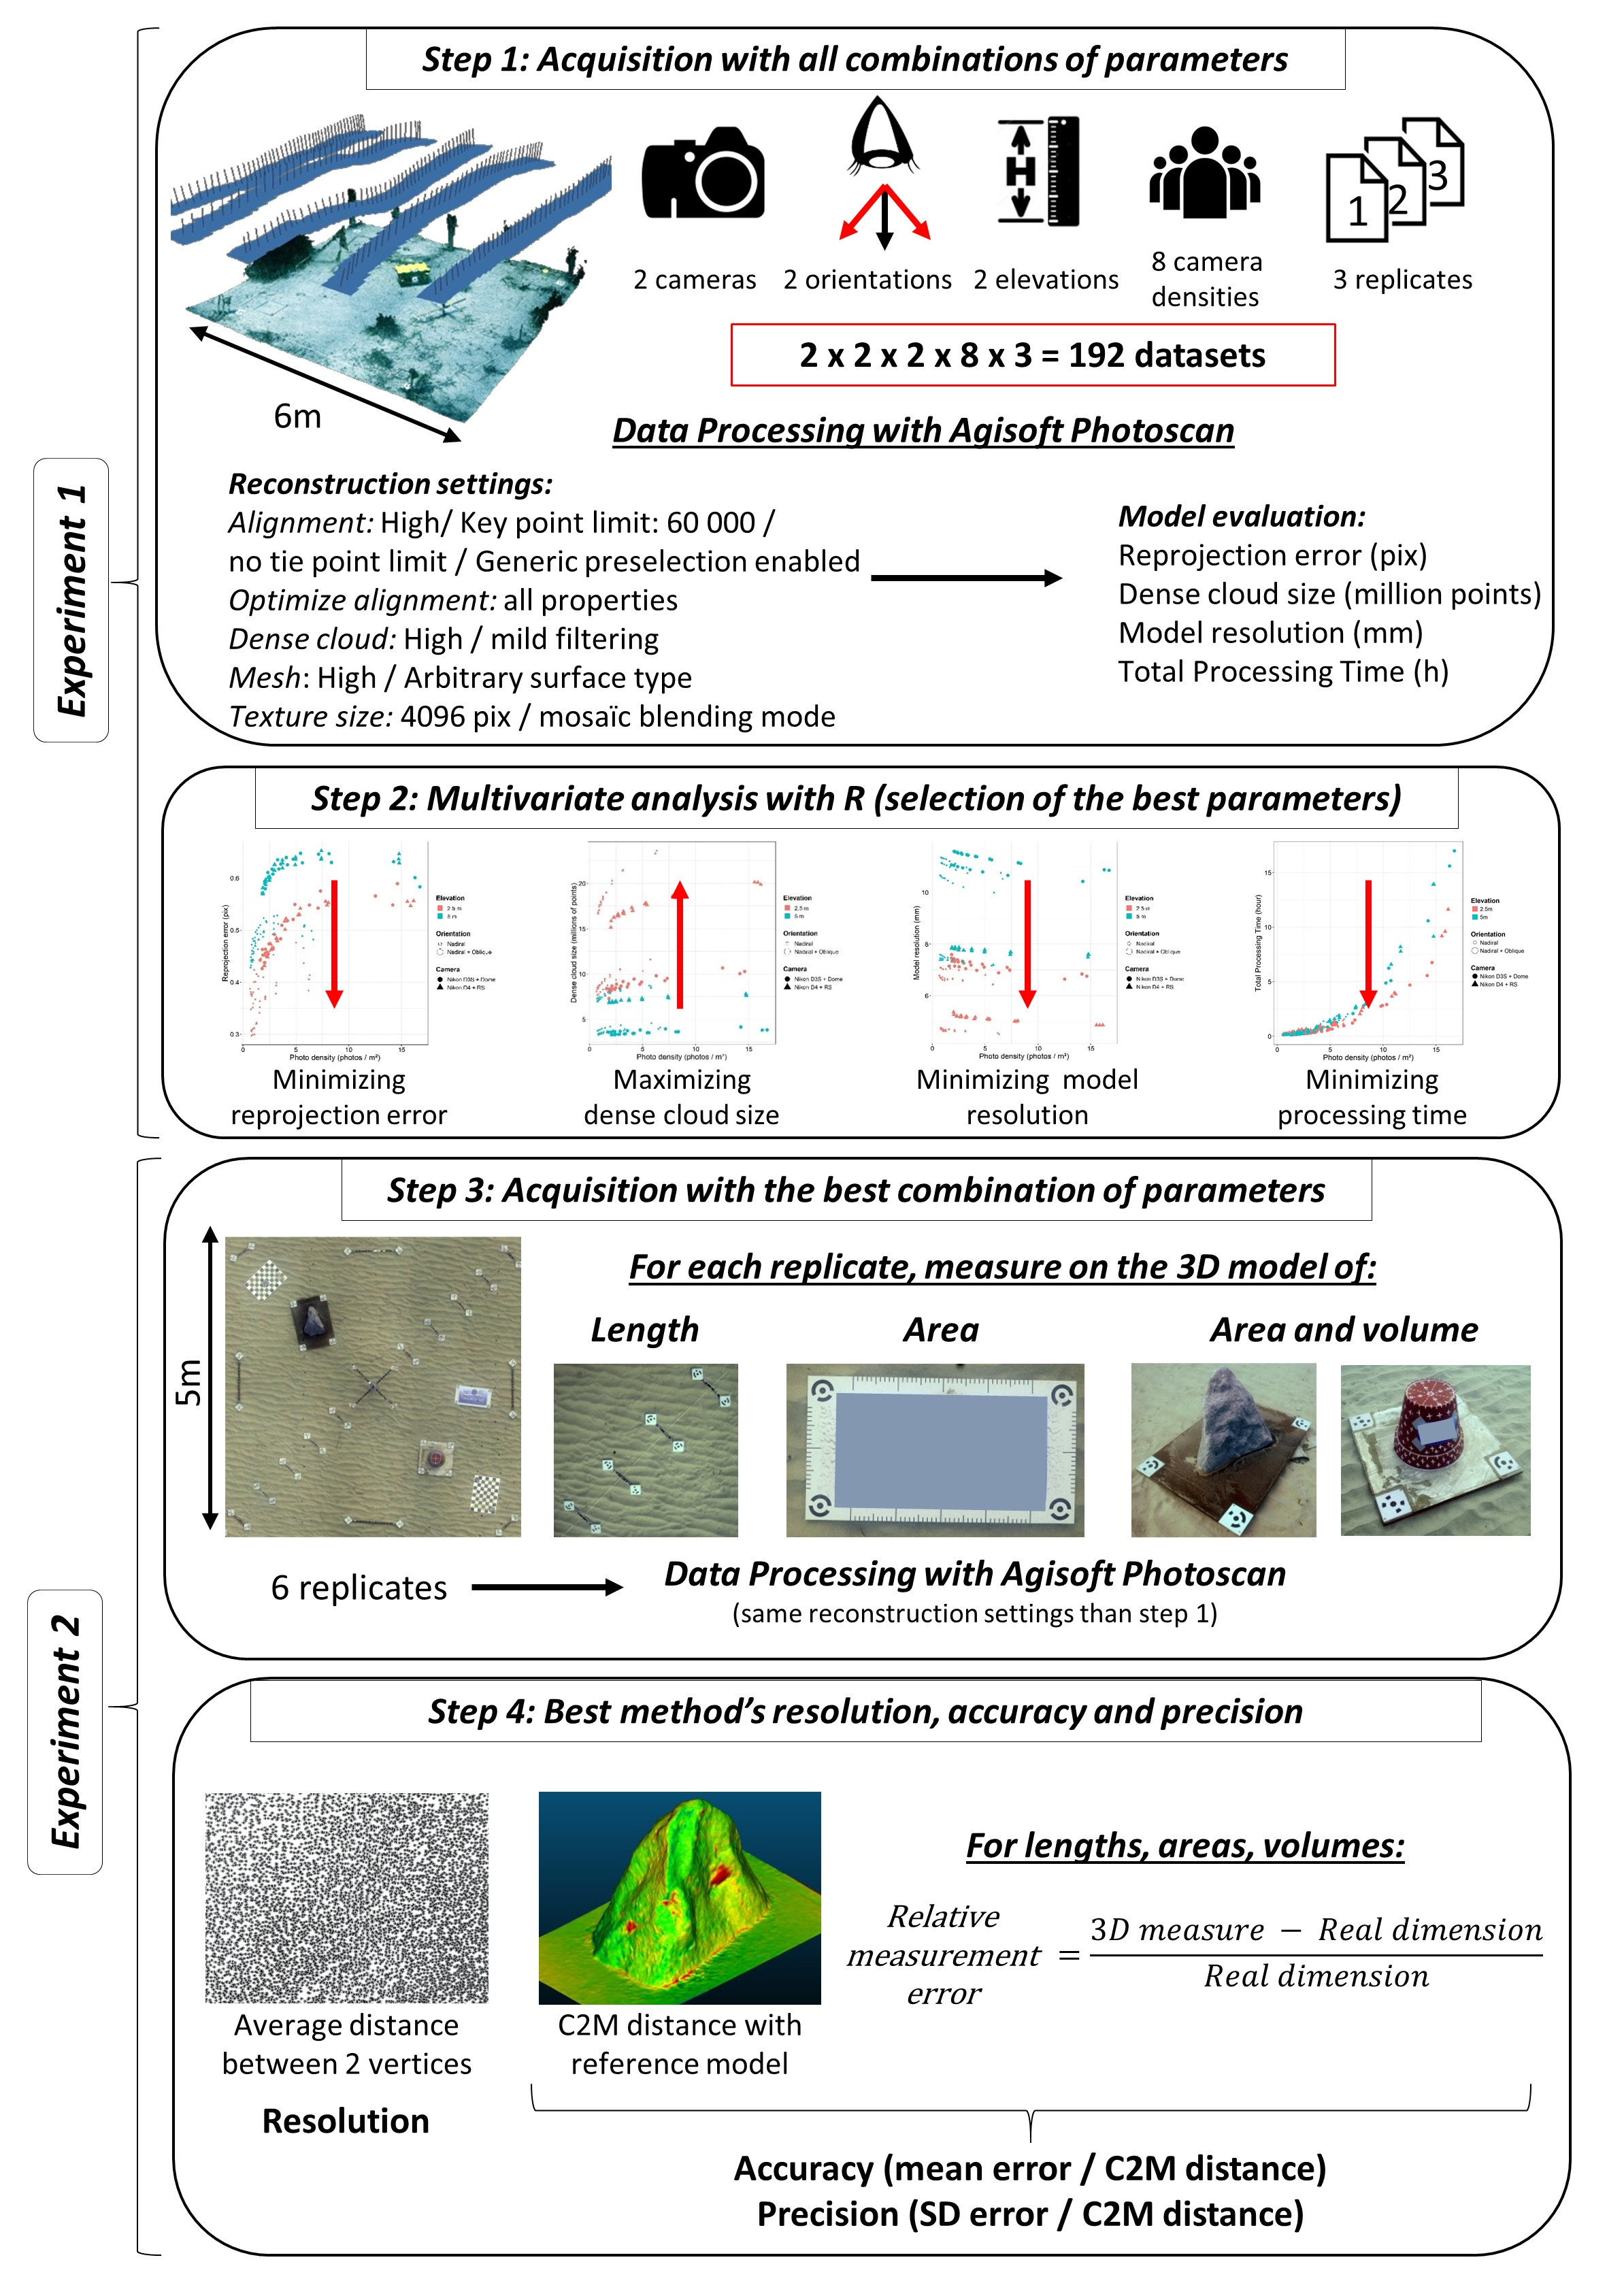
\includegraphics[width=\linewidth]{./4_chapitre2/Figure2.1.jpg}
		\caption[Flow diagram of the methodology.]{Flow diagram of the methodology. \textit{C2M = Cloud-to-mesh.}}
	\label{figure2.1}
	
\end{center}
\end{figure}

\subsection{Experimental design}\label{chapitre2_2.1}

\subsubsection{Experiment 1: defining the best set of parameters for acquisition}\label{chapitre2_2.1.1}

The first experiment tested different combinations of parameters, assessing their relative effects on the accuracy of bundle adjustment and model resolution. The experiment took place at 15 m depth in the Mediterranean Sea (Calvi bay, Corsica, France) and corresponded to a 6 x 6 m patch of sand in between dense Posidonia oceanica meadows, with a mixture of existing artificial structures and objects placed across the area. All acquisitions were conducted using two different cameras: 

\begin{itemize}[leftmargin=*]
\item A Nikon D3S in a waterproof Seacam housing, mounted with a Nikon 20 mm fixed lens and a hemispherical dome port (hereafter referred to as “Nikon D3S + Dome”, see details Table \ref{table2.1})
\item A Nikon D4 in a waterproof Seacam housing, mounted with a Nikonos RS 20 - 35 mm marine lens (hereafter referred to as “Nikon D4 + RS”, see details Table \ref{table2.1})
\end{itemize}

%%%%%%%%%%%%%%%%%%%%%%%%%%%%%%%%%%%%%%%%%%%%%%%%
%%% Table 2.1: Camera systems specifications %%%
%%%%%%%%%%%%%%%%%%%%%%%%%%%%%%%%%%%%%%%%%%%%%%%%
% http://mirrors.standaloneinstaller.com/ctan/macros/latex/contrib/booktabs/booktabs.pdf
\begin{table}[H]
  \centering
  %% \tablesize{} %% You can specify the fontsize here, e.g., \tablesize{\footnotesize}. If commented out \small will be used.
  \normalsize
%  \raggedright
  \caption{Camera systems specifications.}
  \label{table2.1}
%  \resizebox{\textwidth}{!}{
    \begin{tabular}{lcc} % left, center, center
        \toprule
        \textbf{}	& \textbf{Nikon D3S + Dome}	& \textbf{Nikon D4 C RS}\\
        \midrule
        Sensor type		& CMOS			& CMOS\\
        Sensor size (mm)		& 24 x 36			& 24 x 36\\
        Pixel size ($\mu$m)     & 8.4       & 7.3\\
        Resolution (Mega Pixels, MP)		& 12.1			& 16.2\\
        Image size		& 4256 x 2832			& 4928 x 3280\\
        Image ratio		& 3 / 2			& 3 / 2\\
        Lens and mounting		& \makecell[c]{Nikon 20 mm fixed lens \\ + hemispherical
        dome port}			& \makecell[c]{Nikonor 20–35 mm \\ marine lens}\\
        \bottomrule
    \end{tabular}
%    }
\end{table}

The diver flew at two different elevations over the horizontal area (2.5 m and 5 m above the seafloor, following a depth gauge), describing parallel and regularly spaced transects, commonly known as the “mow the lawn” method \citep{pizarro_simple_2017}. He flew at a relatively low speed of 20 - 25 m / min with a time lapse of 0.5 s between pictures. Each acquisition was done in two steps: i) a first with nadiral orientation (i.e vertical downwards) and ii) a second with oblique orientation. Nadiral acquisition involved a single path along each transect, and oblique acquisition involved two paths per transect (one towards right, and the other towards the left). Oblique photos were taken with an angle of approximately 30° from vertical.

All combinations of parameters (camera, elevation and orientation) were performed with three replicates per combination, to distinguish intrinsic and extrinsic variabilities. In total, this represents 24 photo datasets. For each dataset, eight sub-datasets were generated by uniformly sampling one over N images ($1 \leq N \leq 8$) to study the effect of photo density on the accuracy of bundle adjustment and model resolution. We ran all models with 100 \%, 50 \%, 33 \%, 25 \%, 20 \%, 17 \%, 14 \%, and 12.5 \% of photos, which represents a total of 192 models ranging from 23 to 594 photos (see step 1 in Figure \ref{figure2.1}). For a given subsampling level (\%), datasets constituted of both nadiral and oblique photos, by definition, resulted in higher camera densities than pure nadiral. All models were orientated and sized with a 1 x 1 m cross scale bar located in the centre of the study area, and were aligned together with four 10 x 10 cm coded markers placed at the corners. The scale bar length was of the same magnitude as the edge of the scanned area (1 m vs 6 m) \citep{vdi/vde_optical_2002}. All models were produced within the same spatial extent (i.e same bounding box), defined by the positions of the four markers placed at the corners of the study site.

Camera settings were adjusted to achieve a sufficient balance between depth of field, sharpness, and exposure, with the constraint of a high shutter speed to avoid image blurring (20 mm focal length, F10, 1 / 250 s, ISO 400). Focus was set automatically at the beginning of each acquisition, then turned to manual.

\subsubsection{Experiment 2: measuring the accuracy and precision with the best set of parameters}\label{chapitre2_2.1.2}

The aim of the second experiment was to evaluate the accuracy and precision of the models by assessing the variability in the positioning of coded markers, and comparing measurements and 3D geometries of true and modelled objects, using the best combination of parameters obtained in experiment 1. The site was located at 15 m depth in the Mediterranean Sea (Roquebrune Bay, next to Cap Martin, France) and corresponded to a 5 x 5 m sandy area, equipped with objects of known dimensions. These include a resin-made fake rock (surface area = 1.04 m\textsuperscript{2}, volume = 20.03 L), a plant bucket (surface area = 0.191 m\textsuperscript{2}, volume = 10.81 L), a 0.6 x 0.4 m pane (surface area = 0.24 m\textsuperscript{2}), ten 0.35 m bars, and four 0.85 m bars (see Figure \ref{figure2.2}). All these objects were tagged with 10 x 10 cm coded markers which were automatically detected by the reconstruction software with a subpixel accuracy. Their 3D position was exported for assessing the XYZ position and bar length measurements. Four coded markers fixed on a 0.9 x 0.9 m cross were used to scale and orientate the models. Additional coded markers were used at the corners of the study site, rock and bucket to automatically set the corresponding bounding boxes, thereby ensuring that the extent for all the global models and rock / bucket sub-models (separate models of the rock and bucket built for area, volume and cloud-to-mesh distance measurements) were identical. Six replicates were acquired with the best combination of parameters concluded from experiment 1 (camera system, flying elevation, camera orientation and photo density) (see step 3 in Figure \ref{figure2.1}).

\subsection{Models processing and camera calibration}\label{chapitre2_2.2}
All models were processed with Agisoft PhotoScan Professional Edition V. 1.4.0 (Agisoft LLC, 2018). This commercial software is commonly used by the scientific community \citep{burns_integrating_2015, burns_utilizing_2015, figueira_accuracy_2015, burns_assessing_2016, guo_accuracy_2016,   casella_mapping_2017, mizuno_simple_2017} and uses a classic photogrammetric workflow. This consists in the automatic identification of key points on all photos, bundle adjustment, point cloud densification, mesh building and texturing. We used the self-calibration procedure implemented in PhotoScan to be as simple and operational as possible, as it has been shown that the refraction effects at the air-port and port-water interfaces can be absorbed by the physical camera calibration parameters during self-calibration \citep{shortis_calibration_2015}. Calibration optimization was conducted for all properties after bundle adjustment (see step 1 in Figure \ref{figure2.1}).

For the experiment 2, the volume and surface area of the rock and bucket were computed and exported after completing a “hole filling” step to close each sub-model. The models were processed on a Windows 10 workstation with the following specifications: 64bits OS, 128 Gb RAM, 2 x NVIDIA GeForce GTX 1080 Ti 11 Gb, Intel Core i9-7920X 12 CPU 2.9 GHz.

%%%%%%%%%%%%%%%%%%%%%%%%%%%%%%%%%%%%%%%%%%%%%%
%%% Figure 2.2: Study site of experiment 2 %%%
%%%%%%%%%%%%%%%%%%%%%%%%%%%%%%%%%%%%%%%%%%%%%%
\begin{figure}[H]
	\begin{center}
	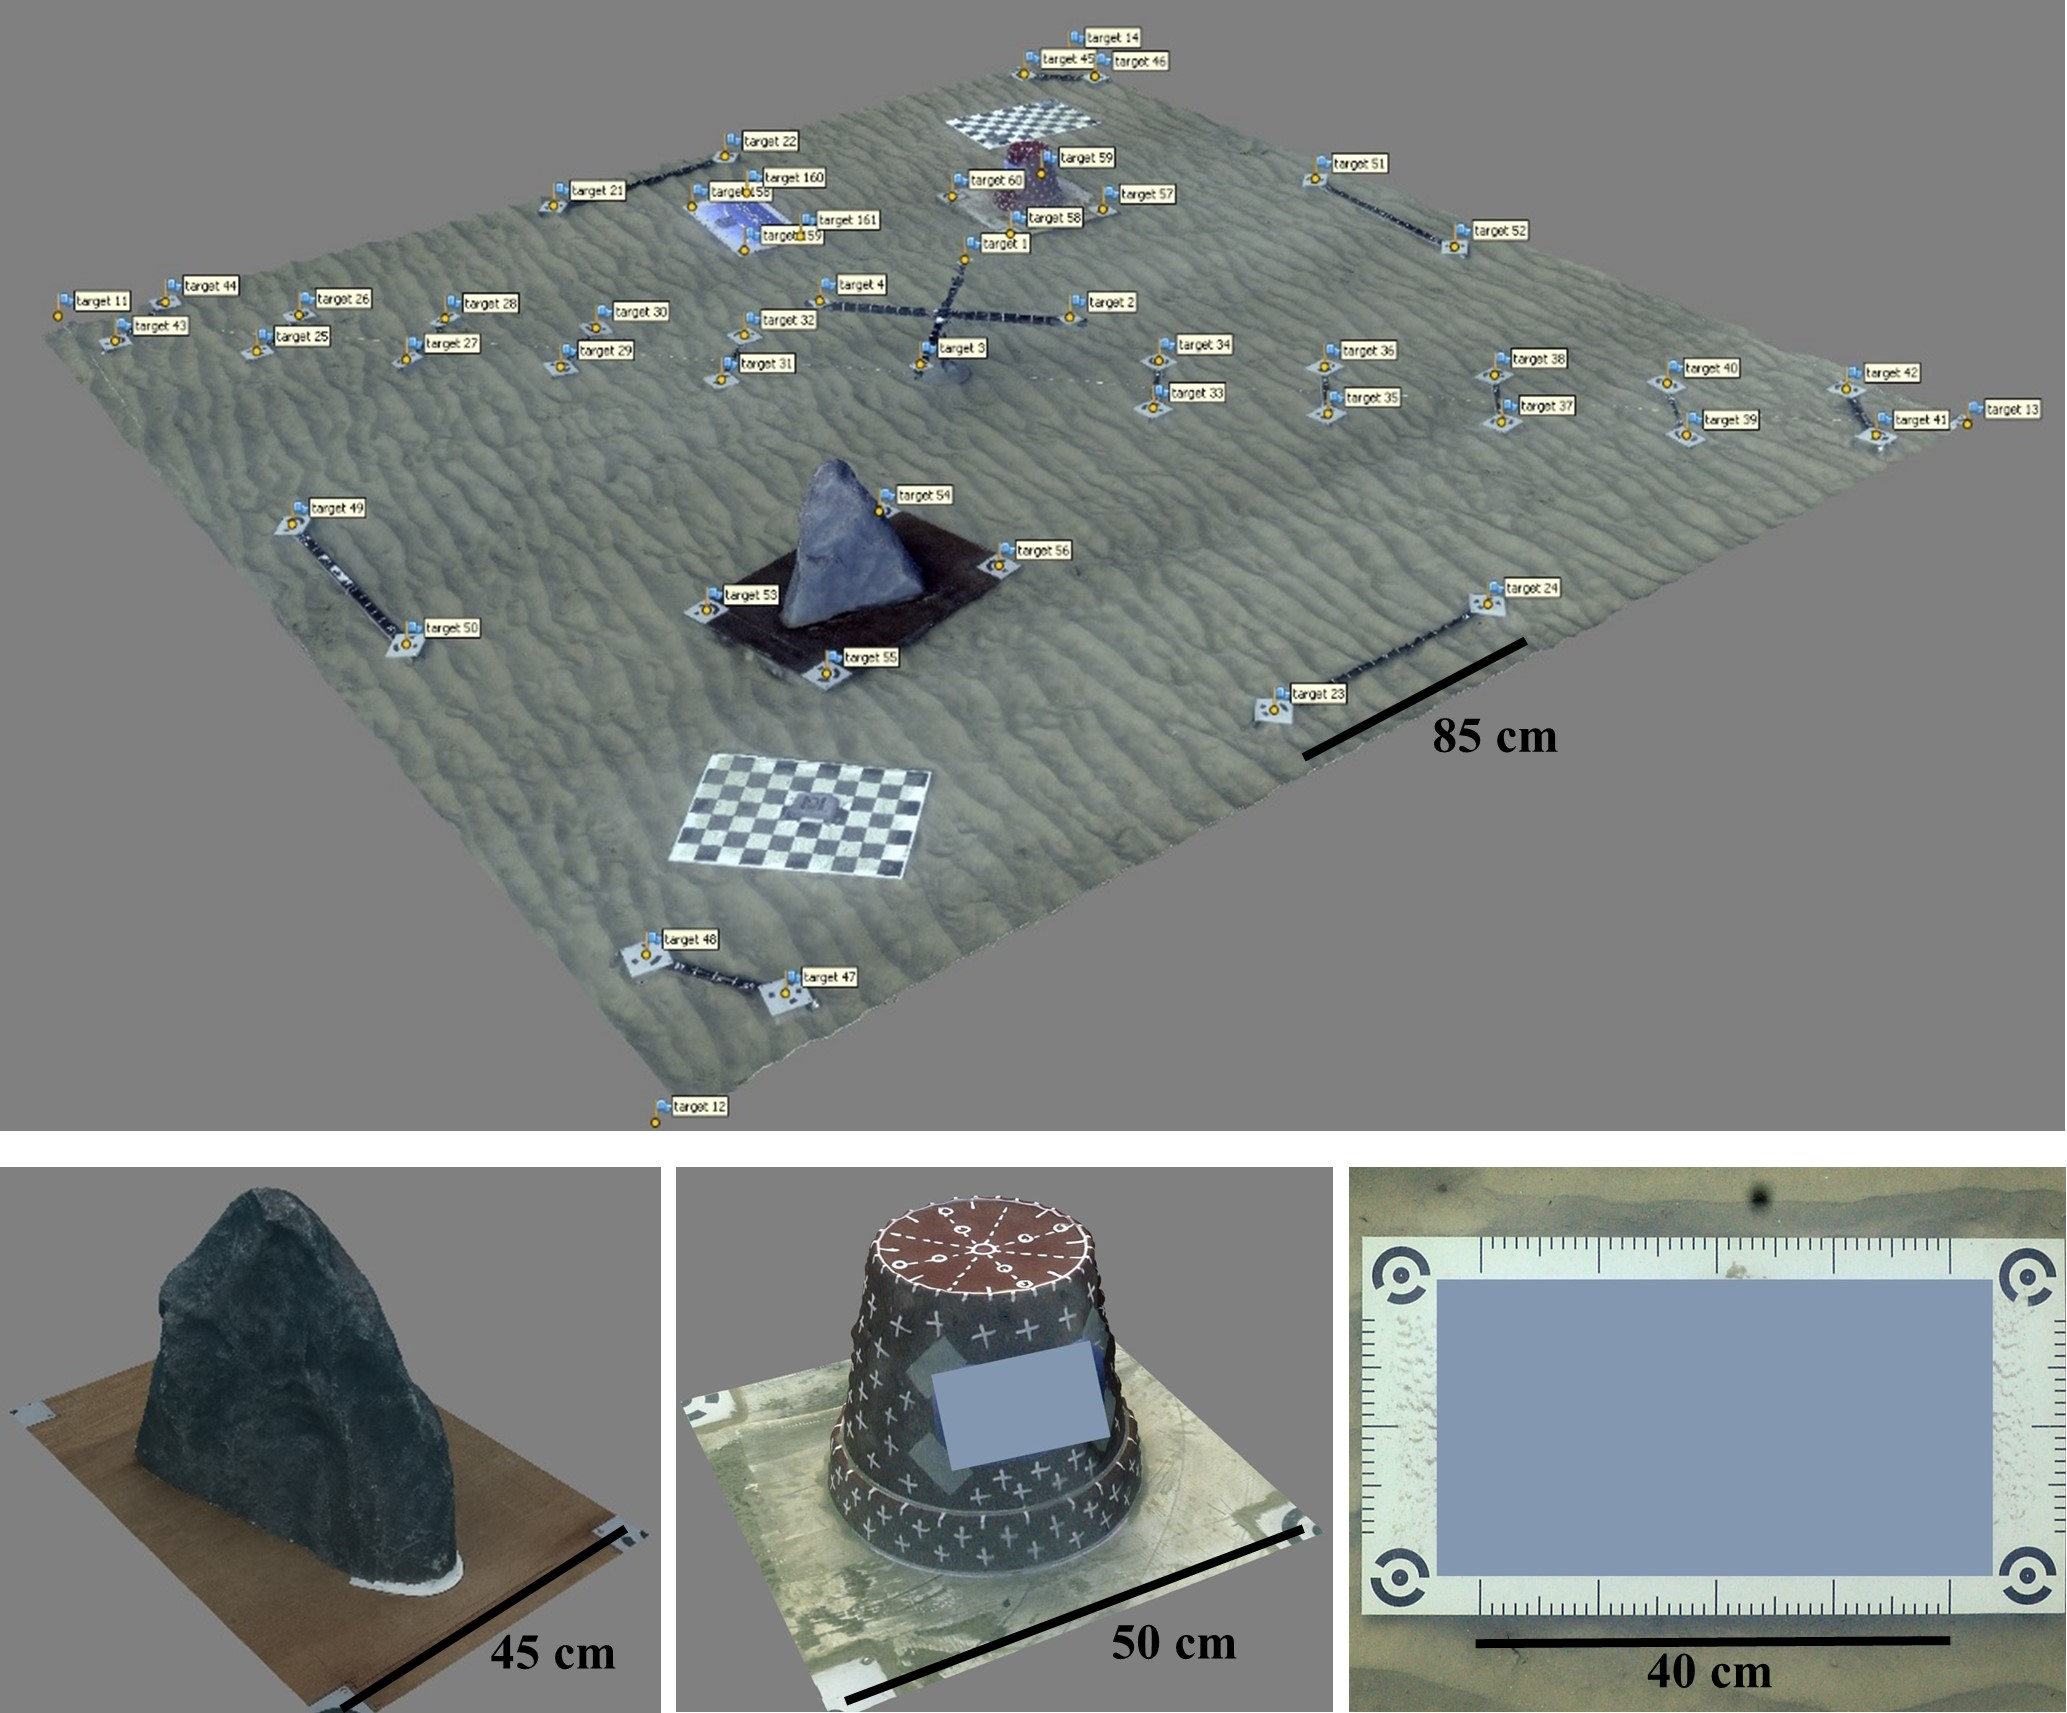
\includegraphics[width=\linewidth]{./4_chapitre2/Figure2.2.jpg}
		\caption[Study site of experiment 2]{Study site of experiment 2, sub-models of the rock, bucket, and the logo pane, with rulers}
	\label{figure2.2}
\end{center}
\end{figure}

\subsection{Metrics}\label{chapitre2_2.3}

\subsubsection{Accuracy of bundle adjustment}\label{chapitre2_2.3.1}
For all processed models, we computed several metrics with a view to assessing the accuracy of bundle adjustment. The reprojection error (see Table \ref{table2.2}) is a good indicator of the quality of self-calibration process during bundle adjustment. The \gls{gcp_rmse} measures the difference between true coordinates of a \gls{gcp} and its coordinates calculated from all photos. The \acrshort{gcp_rmse} / \gls{gsd} gives good indication of the realized vs potential accuracy \citep{forstner_photogrammetric_2016}, as \acrshort{gsd} corresponds to the pixel size in mm (see Table \ref{table2.2}). Experiment 1 aims at minimizing these three metrics to ensure accurate bundle adjustment.

%%%%%%%%%%%%%%%%%%%%%%%%%%%%%%%%%%%%%%%%%%%%
%%% Table 2.2: Definition of the metrics %%%
%%%%%%%%%%%%%%%%%%%%%%%%%%%%%%%%%%%%%%%%%%%%
\begin{table}[H]
  \centering
  \normalsize
  \raggedright
  \caption{Definitions of the metrics used in this study.}
  \label{table2.2}
  \scalebox{0.95}[0.95]{
\begin{tabular}{L{4cm} L{1cm}L{10cm}} \toprule
\textbf{Metric}                                        & \textbf{Unit}  & \textbf{Definition}                                                                                                                                                                                                                                                                        \\
\midrule 
\multicolumn{3}{l}{\multirow{2}{*}{\textbf{Experiment 1: accuracy of bundle adjustment}}}                                                                                                                                                                                                                                                                             \\
\multicolumn{3}{l}{}                                                                                                                                                                                                                                                                                                                                                  \\
Reprojection error                                     & pixels         & Root mean square reprojection error, averaged over all tie points on all images. The reprojection error represents the average distance, in pixels, between a tie point on the image (from which a 3D point has been reconstructed) and the reprojection of its 3D point back on the image. \\
Ground Sample Distance (GSD)                           & mm / pix       & Distance between the centre of two pixels measured on the ground (“pixel size in object space units” (Granshaw 2016)).                                                                                                                                                                      \\
                                                       &                & GSD = (sensor width (mm) x flying elevation (m)) / (real focal length (m) x image width (pix)) for a given image.                                                                                                                                                                           \\
                                                       &                & This value is averaged over all images by PhotoScan and is available in the model processing report (see “Ground resolution” in the “Survey Data” section of the report).                                                                                                                   \\
Ground Control Point Root Mean Square Error (GCP RMSE) & mm             & Root mean square error of the position of a given ground control point across all photos in object space units.                                                                                                                                                                             \\
GCP RMSE / GSD                                         & none           & Ratio of GCP RMSE and GSD.                                                                                                                                                                                                                                                                  \\
\multicolumn{3}{l}{\multirow{2}{*}{\textbf{Experiment 2: accuracy and precision of the models}}}                                                                                                                                                                                                                                                                      \\
\multicolumn{3}{l}{}                                                                                                                                                                                                                                                                                                                                                  \\
XYZ marker positioning                                 & mm             & Standard deviation of the positioning of markers along the three axes (X, Y and Z), across the six replicates.                                                                                                                                                                              \\
Relative measurement error                             & \%             & The accuracy and precision of objects measurements were assessed with the mean and standard deviation of the relative measurement error, respectively.                                                                                                                                      \\
Cloud-To-Mesh distance (C2M)                           & mm             & Absolute distance between a 3D point of the rock model to the in-air reference model.                                                                                                                                                                                                       \\
                                                       &                & The accuracy and precision of 3D geometries were assessed with the mean and standard deviation of the C2M distance, respectively.                                                                                                                                                           \\
\textbf{Model statistics}                              &                &                                                                                                                                                                                                                                                                                             \\
Dense cloud size                                       & million points & Total number of points in the dense cloud.                                                                                                                                                                                                                                                  \\
Model resolution                                       & mm             & Average distance between a vertex of the mesh and its closest neighbour. This value was obtained by averaging the distance between a vertex and its closest neighbour for 10 000 randomly selected vertices.                                                                                \\
Total Processing Time (TPT)                            & hours          & Total processing time for each model: bundle adjustment, point cloud densification, meshing and texturing.\\                                                       \bottomrule
\end{tabular}
    }
\end{table}

\subsubsection{Model statistics}\label{chapitre2_2.3.2}
Since the aim of this study was to define the best trade-off between the development of high-resolution models and the speed of their reconstruction, model resolution and \gls{tpt} were computed for all processed models. Model resolution was defined as the average distance between a vertex of the mesh and its closest neighbour (see Table \ref{table2.2}), and the \acrshort{tpt} including bundle adjustment, point cloud densification, meshing and texturing. In order to take into account model completeness, the dense cloud size (million points) was also calculated.

\subsubsection{Accuracy and precision of the models}\label{chapitre2_2.3.3}
The precision of the positioning of 52 coded markers was assessed by calculating the SD of their XYZ position across the six replicates (see Table \ref{table2.2}). The SD was analysed with regards to the distance to the model centre, to assess a potential decrease in precision for points located further away from the centre. The accuracy of the positioning was not assessed because exact XYZ positions of the markers was not available.

The accuracy and precision of measurements for all objects of known dimensions (lengths, areas, volumes; see step 4 in Figure \ref{figure2.1}) were assessed with the mean and SD of the relative measurement error (see Table \ref{table2.2}). The simple geometry of the bucket allowed for the calculation of its volume and surface area. The rock volume and surface area were measured on an ultra-high resolution, in-air reconstruction \citep{bryson_characterization_2017} using 255 photographs taken with the Nikon D4. The photos were taken from a variety of orientations, using maximum quality parameters for reconstruction. The in-water rock models were aligned to the in-air reference with the four coded markers, and compared using cloud-to-mesh signed distance implemented in CloudCompare Version 2.10 (CloudCompare, GPL software, 2018). The accuracy and precision of the reconstructions were assessed with the mean and SD of absolute distances between the six replicates and the in-air reference (see Table \ref{table2.2}), calculated for 5 000 000 points randomly selected on the reference rock surface.

\subsection{Analysis of the results}\label{chapitre2_2.4}
All marker positions and model statistics were exported from Photoscan as text and PDF files (PhotoScan processing reports). They were parsed and analysed with R Software V. 3.4.2 (R Core Team, 2017). The accuracy of bundle adjustment was assessed using the reprojection error, \acrshort{gcp_rmse} and \acrshort{gcp_rmse} / \acrshort{gsd}. The resolution of the models after densification and meshing was defined as the average distance between two neighbour vertices of the mesh (see \ref{chapitre2_2.3.2}. The individual effect of each parameter (camera system, flying elevation, camera orientation and photo density) on the different metrics (reprojection error, \acrshort{gcp_rmse}, \acrshort{gcp_rmse} / \acrshort{gsd}, dense cloud size, model resolution and \acrshort{tpt}) was evaluated with a \gls{lmm} \citep{zuur_mixed_2009} after a log-transformation was performed to linearize the relationship with photo density. \acrshort{lmm}s are statistical models that are suited for the analysis of clustered dependent data. Indeed, in all models built from the subsampling of one of the 24 datasets from experiment 1 (for studying the effect of photo density on the different metrics) data points are not independent. \acrshort{lmm}s incorporate both fixed (the explanatory factors: camera system, flying elevation, camera orientation, photo density) and random effects used to control for pseudo-replication in the data by taking into account heterogeneity in the relationships between the explained variable and explanatory factors among the datasets \citep{patino_accounting_2013}. The random effects structure depicts the nesting of datasets from the most to the least inclusive (camera > flying elevation > orientation > replicate). Models were fit with the “lmer” function in the “lme4” R library (v. 1.1-21). Each \acrshort{lmm} was first built with all 4 predictors and sequentially pruned by dropping the least significant predictor until all remaining predictors were significant, such that the final \acrshort{lmm}s only included the predictors that had a significant effect on each metric (t-test < 0.05). \acrshort{gsd} was independently used as a predictor of the dense cloud size, model resolution and \acrshort{tpt} in order to integrate both camera and flying elevation effects and make the results generalizable to a broader range of camera systems and flying elevations.

In experiment 1, the aim was to minimize the reprojection error, the \acrshort{gcp_rmse}, the \acrshort{gcp_rmse} / \acrshort{gsd}, the model resolution, and the \acrshort{tpt}, whilst maximizing the dense cloud size. Experiment 2 assessed the accuracy and precision of the reconstructions obtained with the best set of parameters from experiment 1. This was conducted through the analysis of the XYZ positioning of markers, objects lengths, surfaces and volume measurements, and cloud-to-mesh distance between the rock reconstructions and an ultra-high in-air reference model.

\section[Results]{Results}\label{chapitre2_3}
The weather conditions were clear during both experiments (swell < 0.5 m, wind < 5 knots), and the sky was cloudy, ensuring homogenous enlightening at those relatively shallow depths. Water conditions were homogenous, and refraction was supposed constant over time and space during acquisition, as it has been proven to be insensitive to temperature, pressure and salinity \citep{moore_underwater_1976}. The total acquisition time for both nadiral and oblique passes was 5 to 7 minutes for one given combination of parameters (see step 1 in Figure \ref{figure2.1}). All coded markers were well detected by PhotoScan for all models, and all appeared on a minimum of 4 photos.

\subsection{Influence of acquisition parameters on bundle adjustment accuracy and model statistics}\label{chapitre2_3.1}

\subsubsection{Accuracy of bundle adjustment}\label{chapitre2_3.1.1}
The reprojection error ranged from 0.30 to 0.65 pixels across all models, but was significantly smaller at 2.5 m flying elevation and pure nadiral orientation. The proportion of variance explained for the overall reprojection error was 96.7 \% (see Table \ref{table2.3}). All parameters had a significant effect on the reprojection error (t-test, p < 0.001), except camera system (t-test, p > 0.05). 


%%%%%%%%%%%%%%%%%%%%%%%%%%%%%%%%%%%%%%%%%%%%
%%% Table 2.3: Bundle adjustment metrics %%%
%%%%%%%%%%%%%%%%%%%%%%%%%%%%%%%%%%%%%%%%%%%%
\begin{table}[htbp]
  \centering
  \normalsize
 % \raggedright
  \caption[Effects of the acquisition parameters on the bundle adjustment metrics.]{Effects of the acquisition parameters on the bundle adjustment metrics. \textit{N and 0: Nadiral and Oblique; results show the estimate of slope and the p-value of the t-test (“-“if p > 0.05; “*” if p < 0.05; “**” if p < 0.01; “***” if p < 0.001); GCP RMSE = Ground Control Point Root Mean Square Error; GSD = Ground Sample Distance.}}
  \label{table2.3}
%  \resizebox{\textwidth}{!}{
    \begin{tabular}{l c c c}
        \toprule
    
                                         & \textbf{\makecell[c]{Reprojection error \\ (pix)}} & \textbf{\makecell[c]{GCP RMSE \\ (mm)}} & \textbf{GCP RMSE / GSD} \\
    \midrule

    \makecell[l]{Camera system \\ (D4 + RS / D3S + Dome)} & -                                 & -                      & -                       \\
    Flying elevation (unit / m)          & 0.12 ***                          & -                      & -0.22 **                \\
    Orientation ((N+O) / N)              & 0.16 ***                          & -                      & -                       \\
    \makecell[l]{Photo density \\ (unit / photo.m-²)}     & 0.08 ***                          & -0.22 ***              & -0.22 ***               \\
    Variance explained                   & 96.7 \%                           & 64.5 \%                & 67.3 \%
    \\
    \bottomrule
    \end{tabular}
 %   }
    
\end{table}

The \acrshort{gcp_rmse} ranged from 0.1 to 9.0 mm across all combinations, but 83 \% of models had a value smaller than 1 mm (see Figure \ref{figure2.3}). The proportion of variance explained for the overall modelled GCP RMSE was 64.5 \%. The only parameter that had a significant effect on GCP RMSE was the photo density (t-test, p < 0.001, see Table \ref{table2.3}), with a negative trend. 

%%%%%%%%%%%%%%%%%%%%%%%%%%%%%%%%%%%%%%%%%%%%%%%%%%%%%%%%%%%%%%%%%%%%%%%%%%%%%%%%%%%%%%%
%%% Figure 2.3: Bundle adjustment metrics in function of the acquisition parameters %%%
%%%%%%%%%%%%%%%%%%%%%%%%%%%%%%%%%%%%%%%%%%%%%%%%%%%%%%%%%%%%%%%%%%%%%%%%%%%%%%%%%%%%%%%
\begin{figure}[ht]
%	\begin{center}
%    \setlength{\fboxsep}{1pt}%
%    \setlength{\fboxrule}{1pt}%
%    \fcolorbox{bordercolor}{paddingcolor}{image}
%    \fcolorbox{red}{yellow}{\includegraphics[width=0.5\linewidth]{foobarbaz}}
    \frame{
	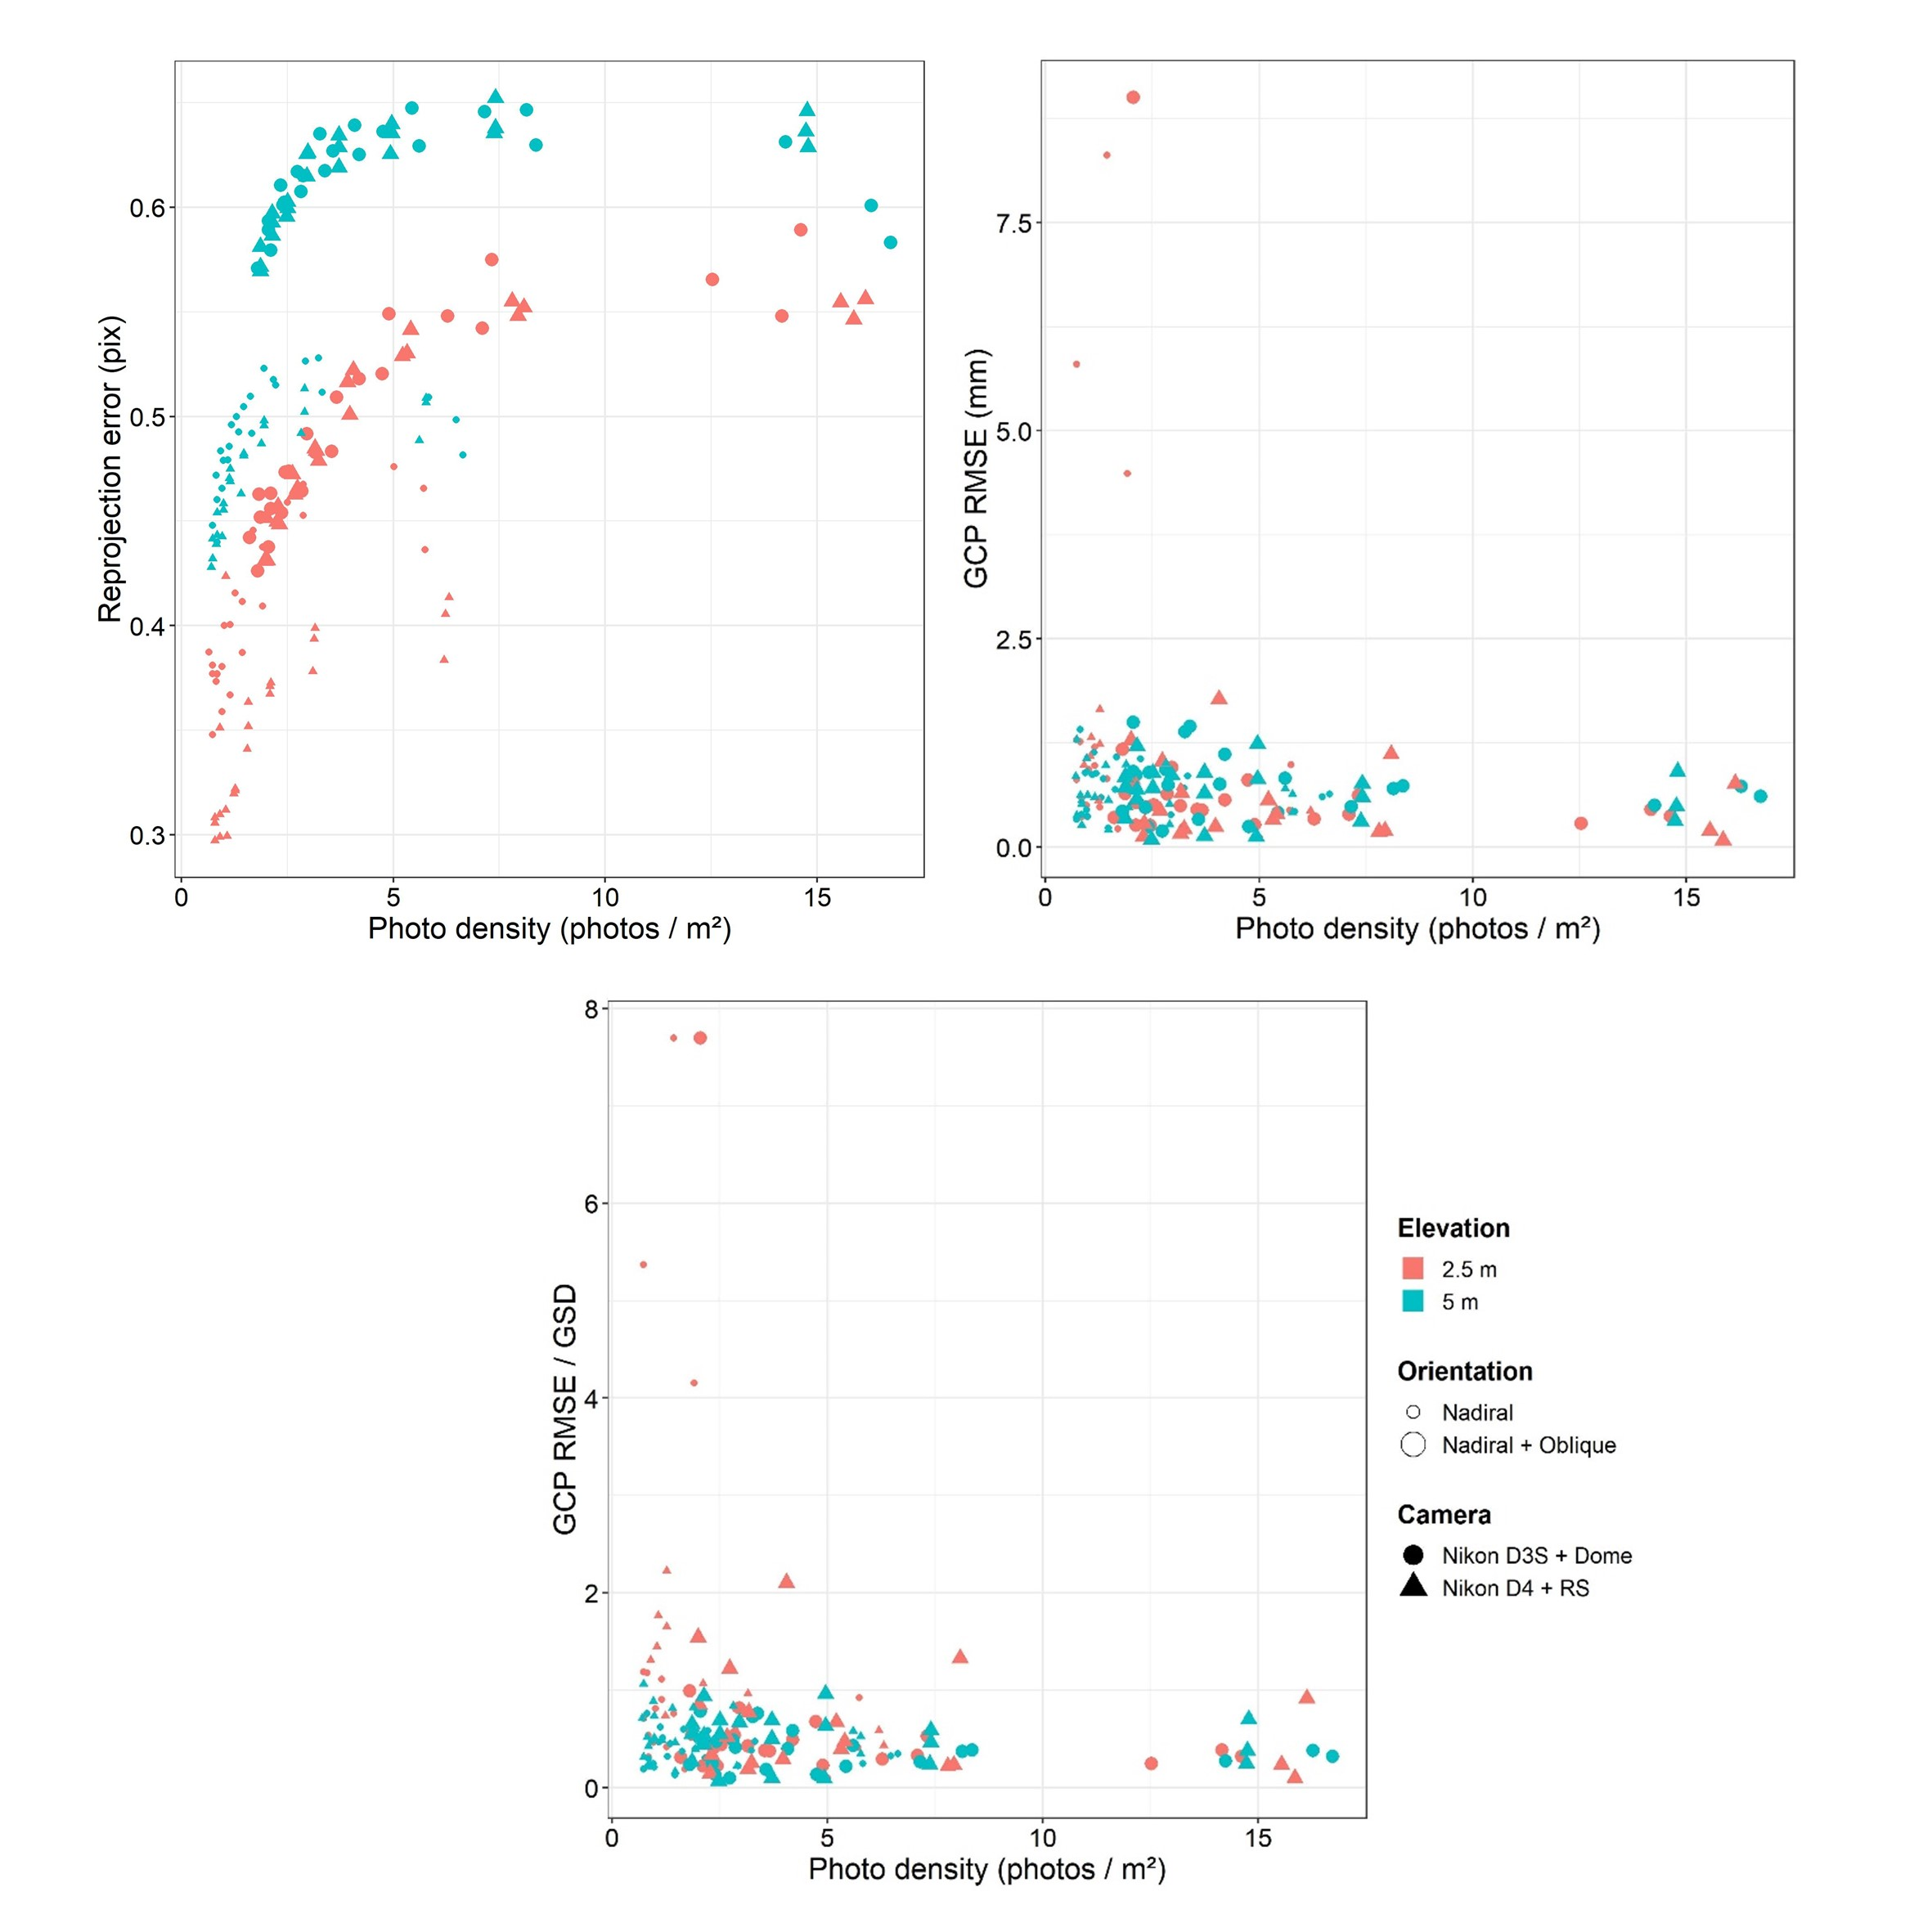
\includegraphics[width=\linewidth]{./4_chapitre2/Figure2.3.jpg}
	}
	\caption[Bundle adjustment metrics in function of the acquisition parameters.]{Bundle adjustment metrics in function of the acquisition parameters. \textit{(A) Reprojection error; (B) GCP RMSE; and (C) GCP RMSE/GSD ratio; GCP RMSE = Ground Control Point Root Mean Square Error; GSD = Ground Sample Distance.}}
	\label{figure2.3}
%    \end{center}
    
\end{figure}

The \acrshort{gcp_rmse} / \acrshort{gsd} ratio ranged from 0.1 to 7.7 across all combinations, but 89 \% of models had a ratio smaller than 1. The proportion of variance explained for the overall modelled \acrshort{gcp_rmse} / \acrshort{gsd} ratio was 67.3 \% Both flying elevation and photo density had a significant effect on the \acrshort{gcp_rmse} / \acrshort{gsd} ratio (t-test, p < 0.01 and p < 0.001, respectively). Camera system and orientation did not have any significant effect (t-test, p > 0.05).
\subsubsection{Dense cloud size}\label{chapitre2_3.1.2}
The dense cloud size ranged from 3.3 to 24.1 million across all models, but was significantly smaller for the Nikon D3S + Dome with 5 m flying elevation and nadiral + oblique orientation (t-test p < 0.001, see Table \ref{table2.4}). The proportion of variance explained for the overall dense cloud size was 99.9 \%. The camera system and flying elevation accounted for 94.0 \% of the total variance. The orientation and photo density had a significant effect on the model resolution (t-test, p < 0.001) but only accounted for 5.9 \% of the total variance. \acrshort{gsd} as single predictor had a significant effect (t-test, p < 0.001) and accounted for 78.3 \% of the total variance. This \acrshort{gsd} effect corresponded to about -0.15 to -0.62 million points / m\textsuperscript{2} per mm.pix\textsuperscript{-1} (log scale). The combination of parameters that gave the highest dense cloud size included the Nikon D4 + RS with a flying elevation of 2.5 m, and pure nadiral orientation (mean 19.4 million points $\pm$ 2.2 SD; see Figure \ref{figure2.4}).

%%%%%%%%%%%%%%%%%%%%%%%%%%%%%%%%%%%%%%%%%%%%%%%%%%%%%%%%%%%%%%%%%%%%%%%%%%%%%%
%%% Figure 2.4: Model statistics in function of the acquisition parameters %%%
%%%%%%%%%%%%%%%%%%%%%%%%%%%%%%%%%%%%%%%%%%%%%%%%%%%%%%%%%%%%%%%%%%%%%%%%%%%%%%
\begin{figure}[ht]
    \frame{
	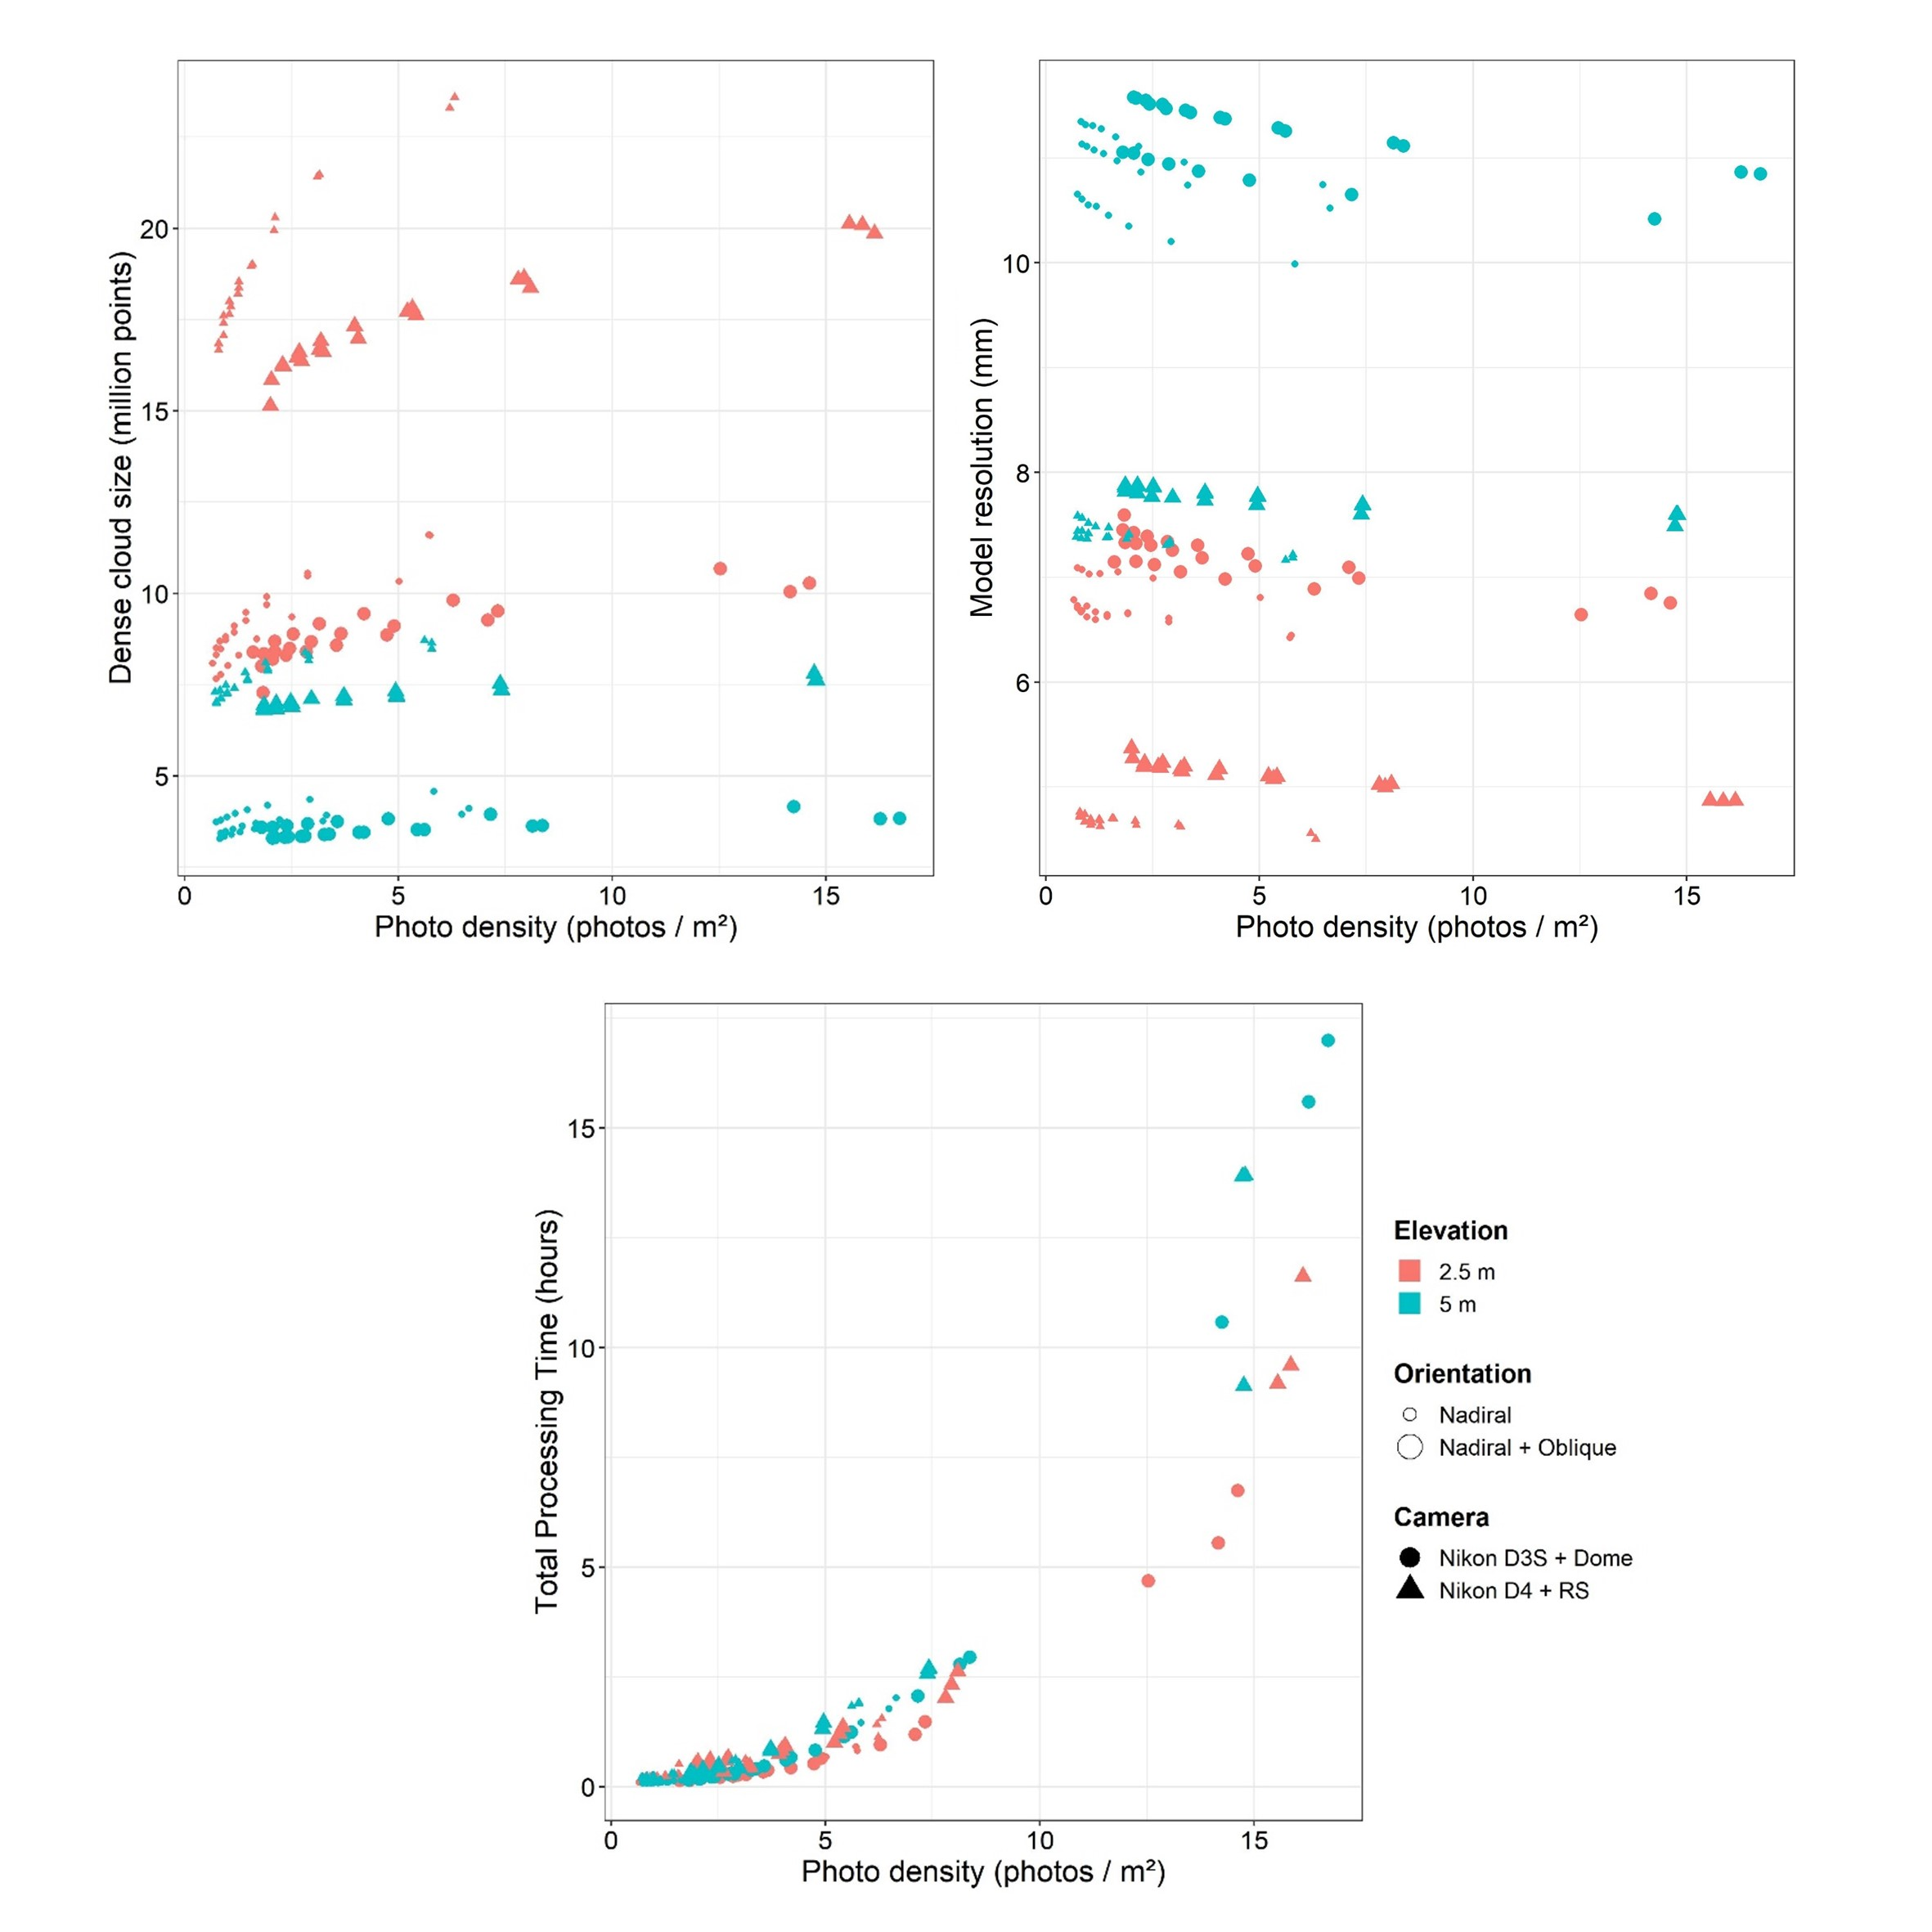
\includegraphics[width=\linewidth]{./4_chapitre2/Figure2.4.jpg}
	}
	\caption[Model statistics in function of the acquisition parameters.]{Model statistics in function of the acquisition parameters. \textit{(A) Dense cloud size; (B) Model resolution; and (C) Total Processing Time.}}
	\label{figure2.4}
	
\end{figure}

The exponential regressions for each combination were in turn calculated (R\textsuperscript{2} = 0.42 - 0.99). Using the regression curves for each combination, the dense cloud size reached 95 \% of the maximum value achieved for a photo density between 3.3 and 18.9 photos / m\textsuperscript{2}, depending on the camera system, elevation, and orientation. For the stated values of photo density, the dense cloud size was 95 \% of the maximum value achieved, and additional photos only increased the number by the remaining 5 \%. The lowest photo density value was obtained from the Nikon D4 + RS camera using pure nadiral orientation at 5 m elevation, while the highest value was obtained from the Nikon D3S + Dome camera using nadiral and oblique orientation at 5 m elevation. The value obtained from the Nikon D4 + RS, 2.5 m altitude and pure nadiral orientation was 4.7 photos / m\textsuperscript{2}.

%%%%%%%%%%%%%%%%%%%%%%%%%%%%%%%%%%%%%%%%%%%%%%%%%%%%%%%%%%%%%%%%%%%%%%%%%%%%%%%%
%%% Table 2.4: Effects of the acquisition parameters on the model statistics %%%
%%%%%%%%%%%%%%%%%%%%%%%%%%%%%%%%%%%%%%%%%%%%%%%%%%%%%%%%%%%%%%%%%%%%%%%%%%%%%%%%
\begin{table}[htbp]
  \centering
  \normalsize
 % \raggedright
  \caption[Effects of the acquisition parameters on the model statistics.]{Effects of the acquisition parameters on the model statistics. \textit{N and 0: Nadiral and Oblique; results show the estimate of slope and the p-value of the t-test (“-“if p > 0.05; “*” if p < 0.05; “**” if p < 0.01; “***” if p < 0.001); TPT = Total Processing Time.}}
  \label{table2.4}
%  \resizebox{\textwidth}{!}{
    \begin{tabular}{lccc}
    \toprule
                                     & \multicolumn{1}{l}{\textbf{\makecell[l]{Dense cloud size \\ (million points)}}} & \multicolumn{1}{l}{\textbf{\makecell[l]{Model resolution \\ (mm)}}} & \multicolumn{1}{l}{\textbf{\makecell[l]{TPT \\ (hours)}}} \\
\midrule
\makecell[l]{Camera system \\ (D4 + RS / D3S + Dome)} & 0.60 ***                                                       & -0.31 ***                                          & 0.55 ***                                 \\
Flying elevation (unit / m)          & -0.46 ***                                                      & 0.23 ***                                           & -                                        \\
Orientation ((N+O) / N)              & -0.10 ***                                                      & 0.05 ***                                           & -0.25 ***                                \\
\makecell[l]{Photo density \\ (unit / photo.m-²)}     & 0.11 ***                                                       & -0.03 ***                                          & 1.43 ***                                 \\
Variance explained                   & 99.9 \%                                                        & 99.9 \%                                            & 91.3 \%                                 
\\
\bottomrule
\end{tabular}
 %   }
\end{table}

\subsubsection{Model resolution}\label{chapitre2_3.1.3}
The model resolution ranged from 4.5 to 11.6 mm across all models but was significantly smaller for the Nikon D4 + RS with 2.5 m flying elevation and nadiral orientation (t-test p < 0.001, see Table \ref{table2.4}). The proportion of variance explained for the overall model resolution was 99.9 \%. The camera system and elevation explained 96.8 \% of the total variance. The orientation and photo density had a significant effect on the model resolution (t-test, p < 0.001) but only accounted for 3.1 \% of the total variance. \acrshort{gsd} as single predictor had a significant effect (t-test, p < 0.001) and accounted for 89.0 \% of the total variance (with log scale). But \acrshort{gsd} and model resolution were linearly positively correlated (Pearson correlation: 0.99), with the following intercept and slope: model resolution = 0.4 + 5.8 mm / mm.pix\textsuperscript{-1}. The combination of parameters that gave the finest model resolution included the Nikon D4 + RS with a flying elevation of 2.5 m, and pure nadiral orientation (mean 4.6 mm $\pm$ 0.06 SD; see Figure \ref{figure2.4}). Model resolution was highly anti-correlated with the dense cloud size (spearman correlation: -0.98).

\subsubsection{Total processing time}\label{chapitre2_3.1.4}
\acrshort{tpt} increased exponentially with the photo density, ranging from 4 min 40 s to 17 hours (see Figure \ref{figure2.4}). \acrshort{tpt} was strongly dependent on the photo density, camera system, and orientation (t-test, p < 0.001, see Table \ref{table2.4}), with 91.3 \% explained variance, but flying elevation was not significant (t-test, p > 0.05). \acrshort{gsd} as single predictor did not have any significant effect (t-test, p > 0.05).

Exponential regressions were calculated for each combination (R\textsuperscript{2} = 0.87 - 0.99). From the regression curves for each combination, it was deduced that the \acrshort{tpt} reached a 5 \% of the overall maximum value for a photo density of 3.8 - 8 photos / m\textsuperscript{2}, depending on the camera system, elevation, and orientation. The lowest photo density values were obtained for Nikon D4 + RS camera at 5 m elevation (for both orientations), while the highest value was obtained for Nikon D3S + Dome camera, pure nadiral orientation and 2.5 m elevation. The value for Nikon D4 + RS at 2.5 m and pure nadiral orientation was 5.0 photos / m\textsuperscript{2}.

\subsection{Accuracy and precision of the models with the best combination of parameters}\label{chapitre2_3.2}
The results stated above show that the best trade-off between high bundle adjustment accuracy, high dense cloud size, high-resolution modelling and low \acrshort{tpt} was achieved using the Nikon D4 + RS camera system at a flying elevation of 2.5 m, using pure nadiral orientation and a targeted photo density of 4 - 5 photos / m\textsuperscript{2} (which corresponds approximately to 1 photo / s at a swimming speed of 20 - 25 m / min). This combination of parameters was used to assess the quality of the models in experiment 2 (six replicates). The average reached photo density was 4.3 photos / m\textsuperscript{2} $\pm$ 0.18 SD over the six datasets with a model resolution of 3.4 mm $\pm$ 0.2 SD. \acrshort{gcp_rmse} on the four markers of the cross scale bar ranged from 0.76 to 0.93 mm.

\subsubsection{Positioning of markers}\label{chapitre2_3.2.1}
The SD of the positioning of 52 markers placed across the modelled area ranged from 0.2 to 1.9 mm in X, 0.2 to 1.8 mm in Y and 0.2 to 4.3 mm in Z (see Figure \ref{figure2.5}). The SD increased with distance to the model centre for all three axes (t-test, p-value < 0.001; see Table \ref{table2.5}).

%%%%%%%%%%%%%%%%%%%%%%%%%%%%%%%%%%%%%%%%%%%%%%%%%%%%%%%%%%%
%%% Figure 2.5: SD of marker coordinates for the 3 axes %%%
%%%%%%%%%%%%%%%%%%%%%%%%%%%%%%%%%%%%%%%%%%%%%%%%%%%%%%%%%%%
\begin{figure}[htbp]
    \frame{
	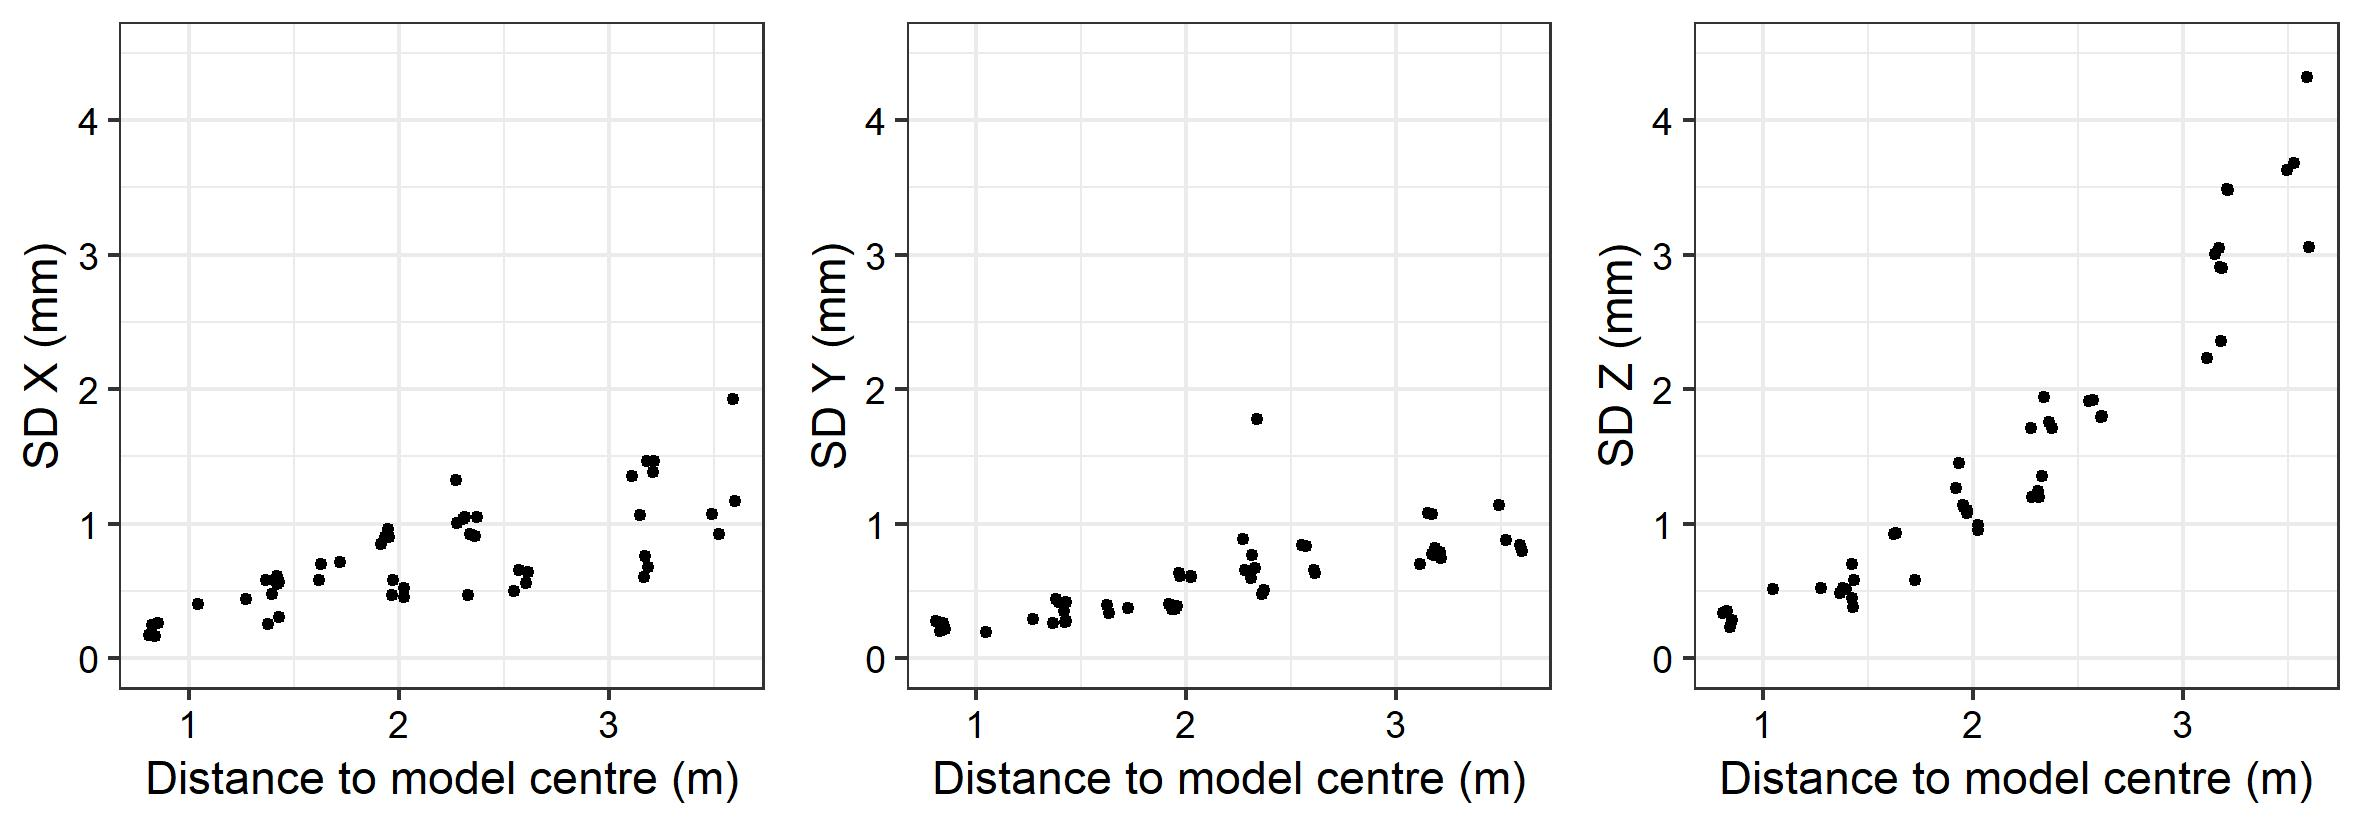
\includegraphics[width=\linewidth]{./4_chapitre2/Figure2.5.jpg}
	}
	\caption[Standard deviation of marker coordinates for the 3 axes]{Standard deviation of marker coordinates for the 3 axes, in function of the distance to the model center. \textit{SD = Standard Deviation.}}
	\label{figure2.5}
\end{figure}



%%%%%%%%%%%%%%%%%%%%%%%%%%%%%%%%%%%%%%%%%%%%%%%%%%%%%%%%%%%%%%%%%%%%%%%%%%%%%
%%% Table 2.5: Effects of the distance to scale bar on marker coordinates %%%
%%%%%%%%%%%%%%%%%%%%%%%%%%%%%%%%%%%%%%%%%%%%%%%%%%%%%%%%%%%%%%%%%%%%%%%%%%%%%
\begin{table}[htbp]
  \centering
  \normalsize
  %\raggedright
  \caption[Effects of the distance to scale bar on the standard deviation of marker coordinates for the 3 axes.]{Effects of the distance to scale bar on the standard deviation of marker coordinates for the 3 axes. \textit{Results show the estimate of slope and the p-value of the t-test (“***” if p < 0.001). SD = Standard deviation.}}
  \label{table2.5}
    \begin{tabular}{@{}llll@{}}
\toprule
                          & \textbf{SD X (mm)} & \textbf{SD Y (mm)} & \textbf{SD Z (mm)} \\ \midrule
Distance to scale bar (m) & 0.33 ***           & 0.27 ***           & 1.2 ***            \\
Variance explained        & 54\%               & 55\%               & 90\%               \\ \bottomrule
\end{tabular}
\end{table}

\subsubsection{Measures of lengths, surfaces and volumes}\label{chapitre2_3.2.2}
The calculation of all measurements was very accurate (mean error < 1 \%, see Table \ref{table2.6}) and precise (SD error < 0.6 \%), except in the case of describing the bucket’s surface area, which indicated a lower accuracy (mean error = 16.11 \%) and precision (SD error = 2.12 \%) (see Table \ref{table2.6}).

%%%%%%%%%%%%%%%%%%%%%%%%%%%%%%%%%%%%%%%%%%%%%%%%%%%%%%%%%%%%%
%%% Table 2.6: Mean and SD of relative measurement errors %%%
%%%%%%%%%%%%%%%%%%%%%%%%%%%%%%%%%%%%%%%%%%%%%%%%%%%%%%%%%%%%%
\begin{table}[htbp]
  \centering
  \normalsize
  %\raggedright
  \caption[Mean and standard deviation of the relative measurement errors for objects contained in the scene]{Mean and standard deviation of the relative measurement errors for objects contained in the scene (experiment 2). \textit{SD = Standard Deviation.}}
  \label{table2.6}
  
      %\scalebox{0.95}[0.95]{
\begin{tabular}{L{4cm} C{2cm}C{2cm}}
        \toprule
                          & \textbf{Mean (\%)} & \textbf{SD (\%)} \\ \midrule
        Bar lengths       & 0.08               & 0.06             \\
        Bucket volume     & 0.06               & 0.25             \\
        Bucket area       & 16.11              & 2.12             \\
        Rock volume       & 0.92               & 0.54             \\
        Rock surface area & 0.36               & 0.51             \\
        Pane area         & 0.26               & 0.04             \\ \bottomrule
    \end{tabular}
%    }
\end{table}

\subsubsection{Reconstruction of 3D geometries}\label{chapitre2_3.2.3}
The in-air model reference of the rock had a resolution of 0.5 mm. The absolute cloud-to-mesh distance between the underwater and the in-air rock model, computed on 5 000 000 randomly selected points, ranged from 0.04 to 9.6 mm across the six replicates (see Figure \ref{figure2.6}). The mean absolute \acrshort{c2m} distance over all points and all replicates was 1.2 mm. The SD of the absolute \acrshort{c2m} distance across the six replicates ranged from 0.01 to 9.5 mm, with a mean value over all points of 0.8 mm. Mean and SD of C2M distance were highly correlated (spearman correlation: 0.77).

%%%%%%%%%%%%%%%%%%%%%%%%%%%%%%%%%%%%%%%%%%%%%%%%%%%%%%%%%%%
%%% Figure 2.6: SD of marker coordinates for the 3 axes %%%
%%%%%%%%%%%%%%%%%%%%%%%%%%%%%%%%%%%%%%%%%%%%%%%%%%%%%%%%%%%
\begin{figure}[htbp]
	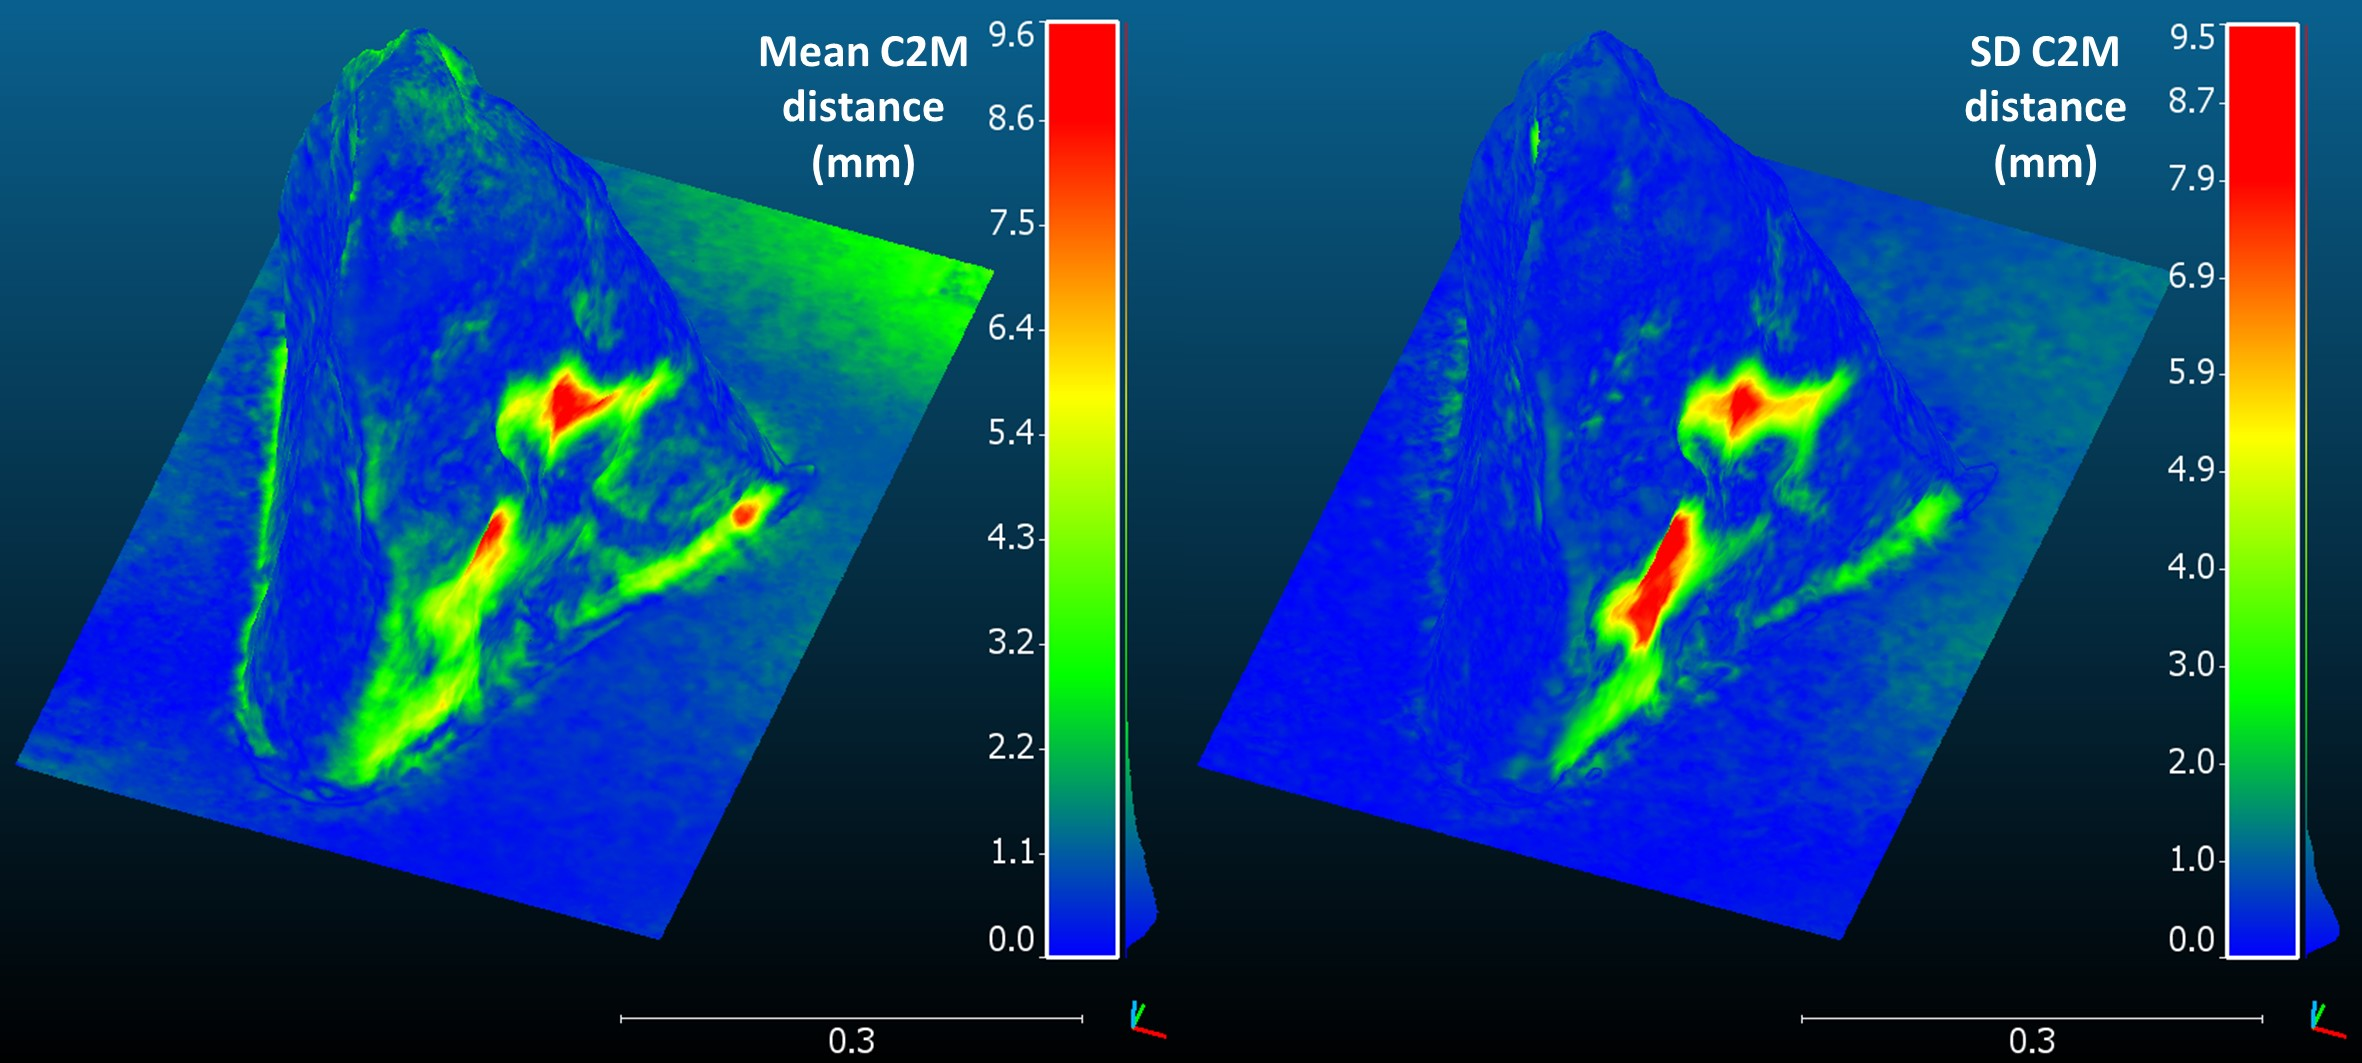
\includegraphics[width=\linewidth]{./4_chapitre2/Figure2.6.jpg}
	\caption[Mean and standard deviation of the absolute cloud-to-mesh distance between the six replicates of the rock model and the in-air reference model.]{Mean and standard deviation of the absolute cloud-to-mesh distance between the six replicates of the rock model and the in-air reference model.\textit{C2M = Cloud-to-mesh; SD = Standard Deviation.}}
	\label{figure2.6}
\end{figure}


\section[Discussion]{Discussion}\label{chapitre2_4}
This study aimed at developing a simple and operational methodology for the 3D reconstruction of marine habitats, with the highest resolution, accuracy and precision, for the shortest processing time. We evaluated the effects of the camera system, flying elevation, camera orientation, and photo density on the resulting reconstructions of a 6 x 6 m sand patch using reprojection error, \acrshort{gcp_rmse}, model resolution, and total processing time. By considering the parameters which gave the best results, and the photo density which achieved the best trade-off between accuracy of the reconstructions and processing time, this study assessed the expected accuracy and precision of reconstructions on a second study site with reference objects of known dimensions and geometry.

\subsection{Best practices for underwater photogrammetry}\label{chapitre2_4.1}
The bundle adjustment was mostly accurate across all combinations, with a reprojection error no greater than 0.65 pixels and a \acrshort{gcp_rmse} / \acrshort{gsd} ratio smaller than one for 89 \% of the models. This ratio is a good indicator as it represents the ratio between realized and potential accuracy \citep{forstner_photogrammetric_2016}. It was smaller at higher photo densities, indicating that photo density gives more robustness during bundle adjustment. The reprojection error increased with photo density (t-test, p-value < 0.001), but there was a saturation point around 5 - 7 photos / m\textsuperscript{2} with a lower slope for higher densities. Indeed, the reprojection error naturally increases at low photo densities, as with very few photos it is expected that 3D points are reconstructed from only 2 - 3 images and thus have a null or low reprojection error. Flying elevation and nadiral + oblique orientation showed higher reprojection error, due to a lower sharpness of images taken in these configurations. The camera system did not have any significant effect on the reprojection error, which suggests that the self-calibration algorithm implemented in PhotoScan interpreted and corrected the distortions of the two different optical systems fairly successfully. Also, reprojection error is not affected by the sensor resolution as it is expressed in pixel unit.

%\smallskip
The two main drivers of model resolution were the camera system and the flying elevation. The model resolution was in average 2.4 mm smaller for the Nikon D4 + RS (log scale), and 1.8 mm / m elevation. By definition, the \acrshort{gsd} is directly depending on the resolution and size of the camera sensor, and distance to modelled object \citep{forstner_photogrammetric_2016}. Therefore, the closer to the object and the higher the resolution of the sensor, the smaller the \acrshort{gsd}. Model resolution and \acrshort{gsd} being highly linearly correlated (Pearson correlation: 0.99), a smaller \acrshort{gsd} involves a smaller model resolution. Its effect corresponded to 5.8 mm / mm.pix\textsuperscript{-1} (any increase in \acrshort{gsd} by 1 mm leads to an increase of 5.8 mm in model resolution, with quality setting for the dense cloud set to “high”). This is an interesting result to keep in mind when planning a photogrammetric acquisition, as \acrshort{gsd} can be calculated from sensor properties and flying elevation (see Table \ref{table2.2}). For a desired model resolution and a given camera system, one can estimate the corresponding flying elevation to be practiced. However, the quality of the camera system will condition the best possible model resolution, as decreasing the flying elevation would require more and more photos to maintain sufficient overlap between pictures, in turn increasing the overall processing time. Other unpublished experiments undertaken by the participants of this study confirm the impracticality of further decreasing flying elevation in the case of homogenous textures such as muddy sediment or dense seagrass, since the footprints of photos taken at lower elevation can be too small to ensure the reliable capture of key points, confusing the bundle adjustment algorithm. This issue was not observed in the case of biogenic reefs such as coralligenous or coral reefs that exhibit a high number of reliable key points.

%\medskip
On the other hand, dense cloud size was highly anti-correlated with model resolution (spearman correlation: -0.98), hence affected by the same parameters as model resolution, with reverse trends. Indeed, the model resolution was here defined as the average distance between a vertex of the mesh and its closest neighbour. But at low photo densities, the dense cloud size was also impacted by missing surfaces that could not be reconstructed because of the insufficient coverage (mostly at the model edges). This was not observed for photo densities greater than 3 - 4 photos / m\textsuperscript{2}. Taking this effect into account by normalizing by the total area, \acrshort{gsd} had an effect of about -0.15 to -0.62 million points / m\textsuperscript{2} per mm.pix\textsuperscript{-1} (log scale; any increase in \acrshort{gsd} by 1 mm.pix\textsuperscript{-1} leads to a decrease of 0.15 to 0.62 million points per square meter).

%\bigskip
The camera orientation significantly influenced most of the metrics, but most importantly affected the reprojection error. All analyses showed that the best results could be obtained by using pure nadiral orientation rather than nadiral and oblique orientation, contrary to the findings of other studies \citep{chiabrando_influence_2017}. It is nevertheless important to underline the fact that, whilst the selected study sites had a relatively flat topography with low-height objects, in the case of more complex environments such as reefs, oblique images can be vitally important to ensuring the comprehensive analysis of all details of the site. This is illustrated by the cloud-to-mesh distances represented in Figure \ref{figure2.6}: the lowest accuracy and precision corresponded to points located below overhanging parts of the rock that were not always well-represented by the photographs, depending on the exact position of each photo.

\acrshort{tpt} exponentially increased with photo density, necessitating a trade-off between accurate bundle adjustment / high dense cloud size and expected \acrshort{tpt}. It was concluded that a value of 4 - 5 photos / m\textsuperscript{2} of mapped seafloor worked well at 2.5 m height. A higher number of photos would mean that the \acrshort{tpt} would have been considerably higher whilst the accuracy of bundle adjustment and dense cloud size would have seen no such corresponding increase. With 16.2 Mpix, the Nikon D4 required a significantly higher \acrshort{tpt} than the Nikon D3S and its 12.1 Mpix sensor, but this effect was marginal compared to the one of photo density (see Table \ref{table2.4}).

The workflow designed in this study used “high” quality setting for dense cloud generation (see Figure \ref{figure2.1}), which corresponds to a downscaling of the original image size by factor of four (two times by each side, (Agisoft 2018)). However, with this quality level, depth maps and dense cloud generation are the two most time consuming steps of model production (70 – 80 \% of \acrshort{tpt}). A “medium” quality corresponds to a downscaling of the original image size by factor of 16 (four times by each side) and could drastically reduce \acrshort{tpt}. According to the size of the area to be modelled, there could be a trade-off between the \acrshort{gsd} (through flying elevation and sensor properties) and the dense cloud quality in order to reach the desired resolution within the shortest \acrshort{tpt}. At low flying elevation, more photos are required to cover the area, but the \acrshort{gsd} is smaller, which might not require the same quality level as a higher flying elevation in order to reach a given model resolution. Further investigations should tackle this point to help researchers making decisions on this trade-off.

\subsection{Accuracy and precision of the resulting methodology}\label{chapitre2_4.2}
The positioning of markers in the scene was achieved with a SD smaller than 5 mm on the three axes, but was increasing with distance to the centre at a rate of about 0.3 mm / m in XY and 1.2 mm / m in Z. If this precision can be sufficient in many usages, it must be taken into consideration notably in the case of model comparison, such as coral or coralligenous outcrops growth at a reef scale. For such applications, the model should always be centred on the area requiring the finest precision, and changes in Z must be larger than the precision expected at the given distance to reflect true reef changes or growth. This underlines the need for further study at a broader scale so as to evaluate the decrease in precision for areas > 100 m\textsuperscript{2}. People using underwater photogrammetry can place coded markers at the boundaries of the region of interest to assess the lowest expected precision of their models, especially on the Z axis.

However, the methodology achieved a satisfactory accuracy for length measurements, with measurement errors corresponding to 8.0 mm per 10 m. It is important to note that the reference bars used were only 0.35 to 0.85 m long and that the accuracy could be different at larger scales. With regards to volumes and surfaces, the expected accuracy was predicted to decrease with increased object complexity, as informed by several studies \citep{figueira_accuracy_2015, bryson_characterization_2017}. The poorest accuracy and precision occurred in the calculation of the bucket’s surface area. It is quite possible that the texture was too homogenous and that PhotoScan could not identify enough tie points on the surface to build its shape, resulting in important surface artefacts. This must be taken into consideration when monitoring artificial structures with very poor texture such as newly submerged metallic or concrete structures. The reconstruction of the resin-made rock (an imitation of natural surfaces and shapes) on the other hand proved to be very accurate (0.92 \% error for volume and 0.36 \% for area) and precise (0.54 \% SD for volume and 0.51 \% for area), surpassing previous results in similar studies \citep{figueira_accuracy_2015, bythell_three-dimensional_2001, courtney_estimating_2007, gutierrez-heredia_end_2016, lavy_quick_2015, shortis_calibration_2015}. Comparing 3D meshes, the models were also very accurate and precise with a mean C2M distance of 1.2 mm over 5 000 000 randomly selected points on the rock surface, and a SD of 0.8 mm over the six replicates. The highest differences with the in-air reference model were observed for points below overhanging parts of the rock (see Figure \ref{figure2.6}), as they were not always captured by the pure nadiral photos. The highest variability was observed for the same points. Indeed, according to the exact position of photos for each dataset, these points were accurately reconstructed for some replicates, and showed artefacts for others. This highlights the limits of pure nadiral orientation in the case of more complex structures, where the operator should adapt camera orientation to follow the structure of the modelled object.

With the exception of the calculated surface of the bucket, the methodology produced highly accurate and precise reconstructions. The method is well-suited and easily deployed for the study and monitoring of marine benthic ecosystems. Using this method, artificial or natural habitats that exhibit the same level of complexity as the experimental setup (low complexity) could be monitored with an expected 1.2 mm accuracy. Healthy biogenic habitats such as coralligenous and coral reefs are expected to show a high complexity; the accuracy of the method still needs to be assessed for these habitats, as reconstruction errors are known to increase with habitat complexity \citep{bryson_characterization_2017, figueira_accuracy_2015}. This solution is cost-effective and operational in terms of the material resources required for monoscopic photogrammetry, time required underwater, and post-processing time. By comparison, whilst stereoscopic mounts enable the direct scaling of the scene \citep{ahmadabadian_comparison_2013}, they cost twice as much as monoscopic cameras, produce twice as many photos increasing the overall processing time, and do not necessarily achieve more accurate results \citep{figueira_accuracy_2015, abdo_efficiently_2006, bryson_characterization_2017}.

\subsection{Accuracy and precision of the resulting methodology}\label{chapitre2_4.3}
Photogrammetry has been increasingly used for studying and monitoring marine biodiversity (as aforementioned in the introduction). It has been deemed a suitable tool for monitoring natural or anthropogenic disturbances and their effects on biodiversity in marine ecosystems \citep{burns_assessing_2016}. The results of this study showed that, at the small reef scale, photogrammetry can provide very accurate and precise sub-centrimetric reconstructions. 

Biogenic reefs and seagrass meadows are two of the most frequently monitored marine habitats because of the ecological role they play for biodiversity \citep{ballesteros_mediterranean_2006, boudouresque_protection_2012, coker_importance_2014}. Photogrammetry is particularly well suited for the monitoring of reefs as they are built of sessile and immobile organisms, and their 3D structure is known to play a major role in structuring their constitutive ecological assemblages (see introduction). However, artificial light becomes mandatory over 30 - 40 m depth because of light absorption, notably in the case of deeper habitats such as coralligenous reefs \citep{ballesteros_mediterranean_2006}. The methodology outlined by this study can be used to monitor small to medium size reefs (20 – 500 m\textsuperscript{2}); to characterise their structural complexity, measure growth rates and study 3D relationships between species, for example. Given recent developments in deep learning, third-dimensional models can be exploited as an additional information layer for classifying species from their 3D characteristics \citep{maturana_voxnet:_2015, qi_pointnet:_2016}. Models of sub-centimetric resolution are currently confined to use on a small area for practical reasons and computational limitations, but future technological advances might enable use on larger extents. Future research should focus on the use of photogrammetric technology in developing scientific understanding of complex ecological processes related to structure. In the coming years, photogrammetry should support detailed studies covering vast marine regions, opening opportunities to draw correlations with macroecological variables available at a broader scale.


\section[Conclusion]{Conclusion}\label{chapitre2_5}
There has been an increasing demand in recent years for innovative methods capable of easily and efficiently capturing fine-scale ecological processes and detecting small changes for the monitoring of the effects of anthropogenic pressures on marine habitats. This study outlined a method that enables the production of accurate and reproducible, high-resolution models of marine environments with a low total processing time. The simple experimental design supported the test of a set of variables proven operational. All in all, the method is suitable for the monitoring of marine benthic biodiversity in a large-scale multi-sites monitoring system. The study’s results showed that flying elevation and camera system, and therefore ground sample distance, strongly affected the model resolution. Photo density meanwhile vastly influenced processing time and bundle adjustment accuracy. If the operator effect was not studied here, because it indirectly accounts for several factors that are not straightforward (i.e. trajectory, flying elevation, camera orientation, swimming speed, etc), it should be tackled as it could have a major influence, notably at large scales. Accounting for computing limitations, future investigations should assess the accuracy and precision of models built with the same parameters, but at a larger scale (> 500 m\textsuperscript{2}). The influence of the dense cloud quality setting should also be studied as it is expected to play an important role the trade-off between model resolution and total processing time. This study was necessary prior to ecological interpretations of 3D models built with the resulting methodology. 
